\documentclass{article}
\usepackage{color}
\usepackage{tikz}
\usepackage{float}
\usepackage{tabularx}
\usepackage{amsmath}
\usepackage{amssymb}
\usepackage{listings}
\usepackage{enumitem}
\usepackage{syntax}
\usepackage{csquotes}
\definecolor{dkgreen}{rgb}{0,0.6,0}
\definecolor{gray}{rgb}{0.5,0.5,0.5}
\definecolor{mauve}{rgb}{0.58,0,0.82}

\lstset{frame=tb,
  numbers=left,
  stepnumber=1,
  language=Java,
  aboveskip=3mm,
  belowskip=3mm,
  showstringspaces=false,
  columns=flexible,
  basicstyle={\small\ttfamily},
  numberstyle=\color{gray},
  keywordstyle=\color{blue},
  commentstyle=\color{dkgreen},
  stringstyle=\color{mauve},
  breaklines=true,
  breakatwhitespace=true,
  tabsize=2,
  moredelim=**[is][\color{red}]{@}{@},
}

\setlength{\grammarindent}{12em}

\renewcommand{\lstlistingname}{Algorithm}
\newcommand{\tablerow}[4]{ #1 & #2 & #3 & #4\\}
\newcommand{\n}[0]{\\[\baselineskip]}
\newcommand{\qa}[2]{\textbf{Q:} #1 \\ \textbf{A:} #2}
\newcommand{\argument}[4]{\textbf{#1:} #2 \\ \textbf{#3:} #4}

\title{CS3105 AI Notes}
\author{Sizhe Yuen}
\setcounter{tocdepth}{2}

\begin{document}

\tableofcontents

\section{History and Philosophy of AI}
\subsection{The Mechanical Turk}
The Mechanical Turk was a chess playing automaton built in 1770. It was quite good at chess but didn't beat \textit{everybody}. It's creator would always opened the doors and drawers for everyone to see the machinery inside before it started playing.
\begin{figure}[H]
\centering
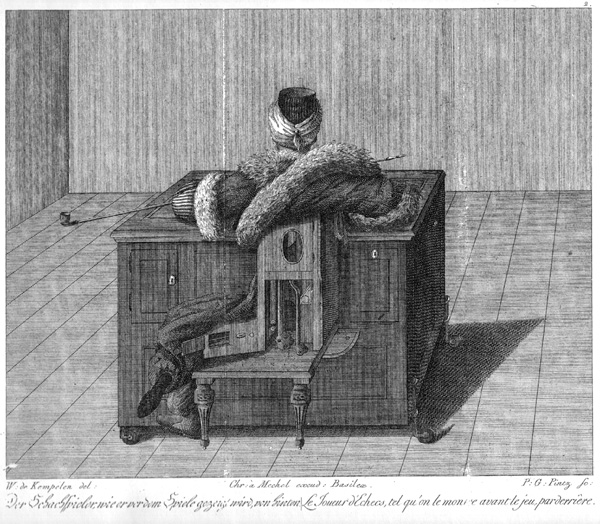
\includegraphics[width=0.8\textwidth, keepaspectratio]{imgs/turk.jpg}
\end{figure}
\noindent
However, this was a hoax as there was actually a small human player hiding inside who moved around inside to hide as different drawers were opened. He could see the moves being made through a magnetic chess set and could make moves by moving the Turk's arms. This was using human intelligence to \textit{fake} artificial intelligence.
\n
Despite being fake, this is an example of people's interest very early in history of Artificial Intelligence.
\subsection{Asimov's Three Laws of Robotics}
The famous science fiction author \textbf{Issac Asimov} developed the \textbf{Three Laws of Robotics} in the 1940s. The laws are as follows:
\begin{enumerate}
\item A robot may not injure a human being or, through inaction, allow a human being to come to harm.
\item A robot must obey the orders given it by human beings except where such orders would conflict with the First Law
\item A robot must protect its own existence as long as such protection does not conflict with the First or Second Laws
\end{enumerate}
\noindent
Artificial intelligence and robots turning on humanity was a popular topic in science fiction novels and Asimov's laws was his take on these plots, not to have the robots ``turn stupidly on [their] creator for no purpose". The laws pose an interesting question in AI ethics. For example the famous trolley ethical experiment of whether one should pull the lever to save five but kill one - what should an AI do given the situation?

\begin{figure}[H]
\centering
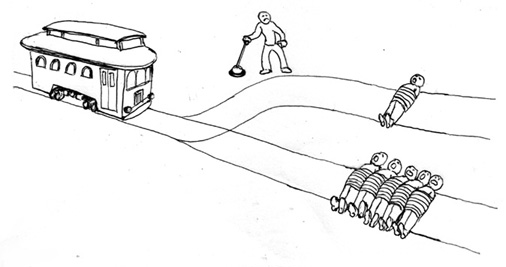
\includegraphics[width=1\textwidth, keepaspectratio]{imgs/trolley.jpg}
\end{figure}
\noindent
Would we program our self-driving cars to kill ourselves in a situation like this?

\subsection{The Turing Test}
In 1950, Turing wrote about what is now called the \textbf{Turing test} and posing the question \textbf{Can Machines Think?} However, instead of answer the question, Turing poses to replace the question by another.
\n
He comes up with what he calls the \textbf{Imitation game}, where a computer has to try to imitate a human so the person talking to it can't tell the difference. In the original paper, the imitation game consists of three people: a man (A), a woman (B) and an interrogator (C). The interrogator stays in a room apart from the other two. The object of the game for the interrogator is to determine which of the other two is the man and which is the woman. A tries to get the interrogator to guess wrong while B tries to help the interrogator. The interrogator is allowed to put questions to A and B. Now he asks the question, ``What will happen when a machine takes the part of A in this game?", ``Will the interrogator decide wrongly as often when the game is played like this as he does when the game is played between a man and a woman?". However he is \textit{not saying} this automatically means the computer can think.
\begin{figure}[H]
\centering
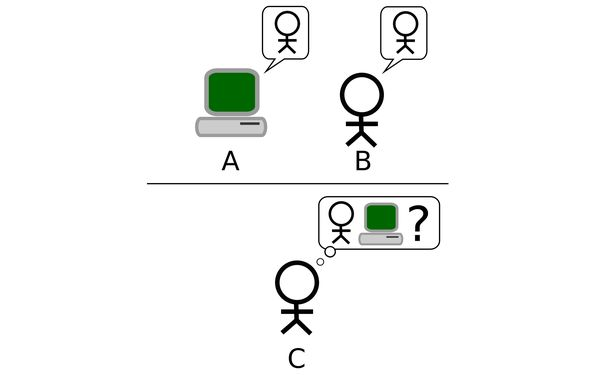
\includegraphics[width=0.8\textwidth, keepaspectratio]{imgs/turingtest.jpg}
\end{figure}
\noindent
Nowadays, the imitation game is usually about whether we can tell if we are talking to a human or a computer, not the man/woman version in Turing's original paper. Turing also had some sample Q\&As on how this should go:
\n
\qa{Write me a sonnet on the subject of the Forth Bridge}{Count me out on this one. I never could write poetry.}
\n
\qa{Add 34957 to 70764}{(Pause about 30 seconds and then give as answer) 105621}
\n
\qa{Do you play chess?}{Yes}
\\
\qa{I have K at my K1 and no other pieces. You have only K at K6 and R at R1. It is your move. What do you play?}{(After a pause of 15 seconds) R-R8 mate.}
\n
The Turing test has been used widely as a test for artificial intelligence and for a long time there has been an annual competition (The Loebner prize) for chat bots. However, the Turing test as been criticized to not properly test of artificial intelligence as people build bots specifically to pass the Turing test (such as \texttt{PARRY}) that are not intelligent at all and instead reflect or play the role of a child or a schizophrenic. 

\subsection{Birth of Artificial Intelligence}
In the summer of 1956, a two-month workshop was organized at Dartmouth College for U.S researchers in the field. This was where the field of AI research was born. Not much was accomplished at the workshop, but for the next 20 years, the people who were there, their student and colleagues at MIT, CMU, Stanford and IBM would dominate the field of AI.
\n 
There were 10 attendees in total, and all were 'superstars' in the field of computer science. This was also where the term \textbf{Artificial Intelligence} first started being used, thanks of John McCarthy.

\subsection{Success, Hubris, Nemesis}
In the history of AI, there has been a common repeated pattern of \textbf{Success $\rightarrow$ Hubris $\rightarrow$ Nemesis}.
\n
\textbf{Success} \\
Something amazing happened, like a breakthrough, or perhaps unrelated that makes everyone think we can do something amazing.
\n
\textbf{Hubris} \\
Something very big and ambitious must be easily achievable thanks to AI and it shouldn't take very long because AI is amazing.
\n
\textbf{Nemesis} \\
It was much harder than we thought and it may not be possible at all. It currently seems like we are in an AI Success/Hubris position again with AI coming up everywhere (AlphaGo, driverless cards etc.), but is this just yet another loop of Hubris/Nemesis?

\subsubsection{Maching Learning}
\textbf{Success} \\
1943 - Neural networks proposed by McCulloch and Pitts \\
1951 - Marvin Minsky built first artificial neural network \\
1957 - Frank Rosenblatt invented the \textit{perceptron} and was able to teach it to learn some boolean functions
\n
\textbf{Hubris} \\
With artificial neurons we should be able to do anything, since they were inspired by the brain so we can just simulate the brain and then we've built an artificial brain!
\n
\textbf{Nemesis} \\
Minsky and Seymour Papert wrote a book \textit{Perceptrons, 1969} which argued that neural networks were limited in scope, including some impossibility theorems. This led to neural network research moribund for the next 15 years.
\n
However now since the invention of back propagation by Werbos, neural networks are a big part of machine learning (for example AlphaGo) and again we have success and hubris for the potential that neural networks can achieve.

\subsubsection{Automated Reasoning}
\textbf{Success} \\
In 1956, Newell, Simon and Shaw were working on a logic theorem prover that proved some of the theorems in ``Principia Mathematica". Not all the theorems were proved, but the approach seemed valid. 
\n
\textbf{Hubris} \\
In 1959, Newell, Simon and Shaw generalised their approach from logic to all problems to create a``General Problem Solver" using a similar approach as their logic machine in the hopes it can solve \textit{any} problem.
\n
\textbf{Nemesis} \\
The General Problem Solver never solved anything interesting as the combinatorial explosion was just too big and they did no have good heuristics. Many of the theorems in Principia were still not solved as well.

\subsubsection{Games Playing}
\textbf{Success} \\
In 1959, Arthur Samuel produced a learning checkers program with techniques like minimax and alpha-beta that beat a ``master" player. 
\begin{figure}[H]
\centering
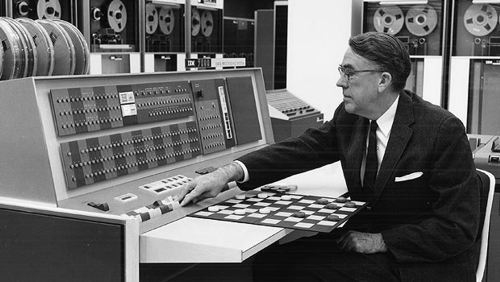
\includegraphics[width=0.8\textwidth, keepaspectratio]{imgs/samuel.jpg}
\end{figure}
\noindent
\textbf{Hubris} \\
It looked like games playing had been cracked, if a computer could beat a human in checkers, surely it would apply to all other games easily. People predicted in 10 years a computer would beat the world chess champion.
\n
\textbf{Nemesis} \\
Chess was a much more complicated game that took longer to solve. Additionally, computers playing Go were horrible due to the large search space and other games like Bridge and Poker were also bad.
\n
As we know recently, AlphaGo beat a top Go player in 2016 and Kasparov (Chess champion) was beaten by ``Deep Blue" in 1997.

\subsection{Weak and Strong AI}
\textbf{Weak AI} \\
Weak AI takes the view that computers are power tools that can do things human otherwise do and can be used to study the nature of mind in general. Weak AI are focused on one narrow task, for example chess playing AIs which can only play chess. Most currently existing systems considered to be AI are weak at the moment.
\n
\textbf{Strong AI} \\
Strong AI takes the view that a computer \textit{is} a mind like a human mind. Seale identified a philosophical position he called ``strong AI":
\begin{quote}
\textit{The appropriately programmed computer with the right inputs and outputs would thereby have a mind in exactly the same sense human beings have minds.}
\end{quote}
He also ascribes the following positions to advocates of strong AI:
\begin{itemize}
\item AI systems can be used to explain the mind
\item The study of the brain is irrelevant to the study of the mind
\item The Turing test is adequate for establishing the existence of mental states
\end{itemize}
\textbf{Artificial General Intelligence (AGI)} \\
More recently, there is a second ``strong AI" definition as an artificial general intelligence which is a machine with the ability to apply intelligence to any problem, rather than just one specific problem and could successfully perform any intellectual task that a human being can. The idea is making an AI system that can do anything.
\n
Ben Goertzel proposed a \textbf{Robot Coffee Test} for AGI. Can you make a robot that can go into any house and make some coffee? The house should be just any ordinary house. This is quite a difficult test as it involves finding coffee, finding water, boiling the water... However, if there is a robot that was built to do this, does it count as AGI? Can the same robot learn how to build a brick wall without being reprogramming?
\n
This leads to an analogy with NP-Complete problems with ``AI-Complete" problems. This implies the difficulty of these problems is equivalent to that of solving the central artificial intelligence problem of creating an AGI. An AI-Complete problem reflects an attitude that it would not be solved by a simple specific algorithm.

\subsection{Attacks on the Turing Test}
There have been many arguments and objections to the Turing Test as a way to signify machine intelligence. Turing himself as responded to many of these objections.
\n
\argument{Theological Objection}{A Man has a soul, machines do not}{Alan Turing}{Can we deny His power to give a soul to a machine?}
\n
\argument{Argument from various disabilities}{No machine can X (e.g. tell right from wrong)}{Alan Turing}{Becomes a less powerful argument each day as machines are capable of doing more as time goes on}
\n
\argument{Lady Lovelace's [Ada's] objection}{Computers do whatever we know how to order them to perform, so computers cannot do anything really new}{Alan Turing}{Machines constantly surprise us}
\n
\argument{Argument from informality of behaviour}{Impossible to write down formal rules for every situation}{Alan Turing}{Impossible to prove people not rule-driven}
\n
\argument{Argument from ESP}{Telepathy would let humans win imitation game}{Alan Turing}{Put competitors in 'telepathy-proof' room}
\n
\argument{Argument from Consciousness}{No mechanism could \textit{feel} pleasure, grief...}{Alan Turing}{Danger of Solipsism(A theory in philosophy that your own existence is the only thing that is real or that can be known)}
\n
\argument{Argument from continuity in the nervous system}{The brain does not operate digitally}{Alan Turing}{Computers can simulate continuous behaviour, e.g. Statistically, graphically, numerically...}
\subsubsection{Godel's theorem}
Godel's theorem states that any consistent and powerful format system must be limited. There must be true statements it cannot prove.
\n
Because computers are formal systems and minds have no limit on their abilities, therefore computers cannot have minds. This point seems to prove that strong AI cannot exist as it certainly applies to computers.
\n
However, Alan Turing had two points to counter this:
\begin{enumerate}
\item \textit{Although it is established that there are limitations to the powers of any particular machine, it has only been stated without any sort of proof, that no such limitations apply to the human intellect}. I.e, it has never been proven that humans have no limitations. Are we sure humans can prove \textit{all} true theorems?
\item \textit{We too often give wrong answers ourselves to be justified in being very pleased at such evidence of fallibility on the part of machines.} Godel's theorem applies only to consistent formal system, however, humans often utter untrue statements, so we might be unlimited format systems which make errors.
\end{enumerate}

\subsubsection{The problem with the Turing Test}
The issue with the actual Turing test is that the chatbots trying to pass the test use \textit{lots of tricks} to try and trick the human on the other end.
\n
For example \texttt{ELIZA} used simple pattern matching:
\begin{itemize}
\item ``Well, \underline{my} boyfriend made \underline{me} come here"
\item ``\underline{Your} boyfriend made \underline{you} come here?"
\end{itemize}
\begin{figure}[H]
\centering
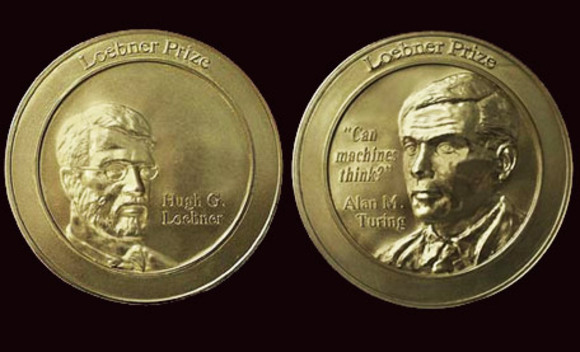
\includegraphics[width=0.8\textwidth, keepaspectratio]{imgs/loebner-prize.jpg}
\end{figure}
Jason Hutchens, who won the Loebner Prize in 1996 wrote an article ``How to pass the Turing test by cheating" where he demonstrated the techniques his chatbot used and how it was not very clever. He also states that ``Turing's imitation game in general is inadequate as a test of intelligence, as it relies solely on the ability to fool people, and this can be very easy to achieve, as Weizenbaum found."
\n
Another example is the 2014 winner, ``Eugene" who posed as a 13-year old, non-native English speaking Ukrainian, which gives lots of ways for judges to explain away his poor English.
\n
Ultimately, whether or not it has been passed, the Turing Test does not drive much AI research.

\subsection{The Chinese Room}
The Chinese Room is one of the most famous attacks on AI. It was created by John Searle. 
\n
The Chinese Room argument holds that a program cannot give a computer a mind or understanding, regardless of how intelligently or human-like the program may make the computer behave. The argument specifically refutes strong AI having a mind like a human being. 
\begin{figure}[H]
\centering
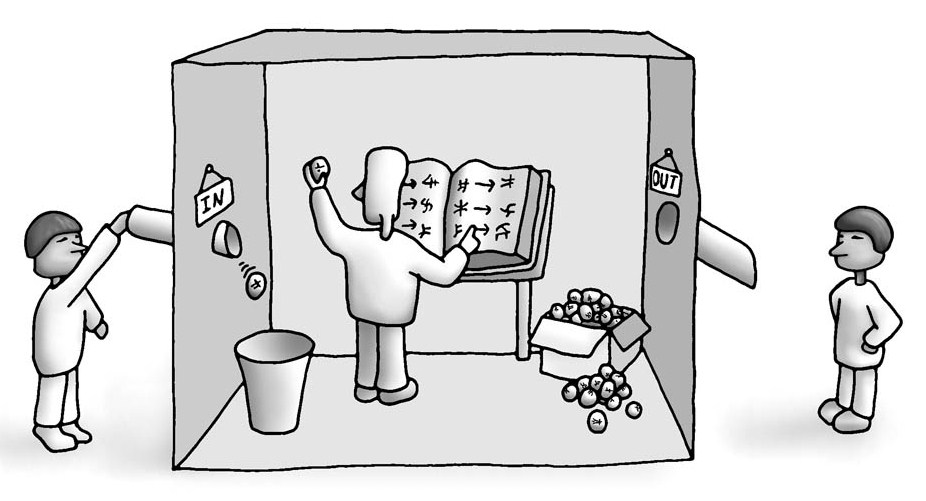
\includegraphics[width=1\textwidth, keepaspectratio]{imgs/chinese-room.jpg}
\end{figure}
\noindent
Suppose there is a computer program that behaves as if it understands Chinese. It can take in Chinese characters as input and by following it's instructions, produce other Chinese characters as output and suppose it was convincing enough to pass the Turing Test: it convinces a human Chinese speakers that the program is itself a live Chinese speaker and to all questions that the person asks, it makes appropriate responses. Searle then asks the question: ``Does the machine \textit{literally} understand Chinese? Or is it merely \textit{simulating} the ability to understand Chinese?" The first would be a strong AI, whereas the latter would be weak AI. Then, the thought experiment is as follows:
\n
Suppose someone is in a closed room with a book in English of the computer program. The person can receive Chinese characters through a slot in the door, process them according to the program's instructions, and produce Chinese characters as output. This is just like running the program manually. The argument is that even though the person is producing behaviour which is interpreted as demonstrating intelligent conversation, the person would \textit{still not be able to understand Chinese} and therefore Searle argues that the computer would not be able to understand the conversation either.
\section{Search}
\subsection{What is search in AI?}
A \textbf{search problem} is defined rigorously. For example it is problems on propositional satisfiability, graph colouring, playing chess etc.
\n
A search algorithm is given an \textbf{Instance} of the problem and the algorithm has to find a \textbf{Solution} to that instance (or report that there is guaranteed to be no solution to that instance or report a timeout if it cannot determine).

\subsubsection{SAT problem}
The boolean SATisfiability problem is an example search problem. An example \textbf{Instance} is a list of words: \texttt{ABC, ABc, AbC, Abc, aBC, abC, abc}. A \textbf{Solution} is a choice of upper/lower case letters where each word must contain at least one of our choices. For example \texttt{AbC}, which is a unique solution to the previous instance.
\n
SAT is a search problem because there is no efficient algorithm known for SAT. In fact, 3-SAT is NP-Complete. 3-SAT is where each word contains exactly 3 letters. Many AI problems fall into the NP-Complete class. DPLL is one of the algorithms to find a solution to that SAT problem. 

\subsubsection{Travelling Salesman problem}
The Travelling Salesman problem is another famous search problem. It involves a salesman travelling across different cities trying to visit each node. An \textbf{Instance} of the problem would be a graph with a cost on each edge and a \textbf{Solution} as a tour visiting all nodes and returning to base or meeting some cost limit. Another variant is to find the minimum possible cost. 

\begin{figure}[H]
\centering
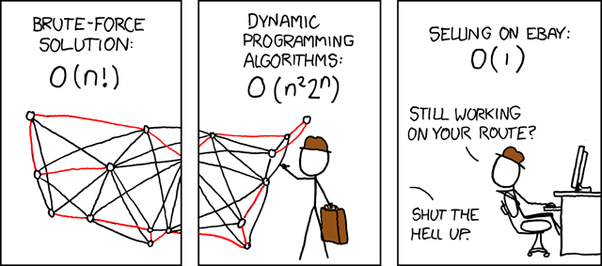
\includegraphics[width=1\textwidth, keepaspectratio]{imgs/tsp.png}
\end{figure}
\noindent
The travelling salesman problem is also NP-Complete if you want to check that the tour costs no more than some limit. A complete solution might need to check every possible path. Of course there are many applications of this problem in real life, especially for delivery companies or moving efficiently around a warehouse for Amazon.

\subsubsection{Games}
Board games like chess and checkers could be thought of as a search problem where the \textbf{Instance} is the current board position of the game and the \textbf{Solution} is a winning strategy from that position. Such games are usually PSPACE-Complete.

\subsection{Presenting Search Abstractly}
There are two main kinds of search algorithm:
\begin{enumerate}
\item \textbf{Complete} search algorithms which are guaranteed to find a solution or prove there is none. Though they may have to be given enough time and so may timeout.
\item \textbf{Incomplete} search algorithms which may not find a solution even if a solution exists. However, these algorithms are often more efficient as they do not have to search through the entire search space.
\end{enumerate}
\noindent
Search states summarise the state of search, in SAT is might be represented by \texttt{aB}. In TSP, a search state might specify some of the order of visits. In Checkers, a search sate might be represented by the board position. With search states we can generalise such to not just finding a solution to a problem.
\n
A \textbf{Search space} is a logical space composed of:
\begin{itemize}
\item \textbf{Nodes} are search states
\item \textbf{Links} are all legal connections between search states
\end{itemize} 
\noindent
Think of a search algorithm as trying to navigate this \textit{extremely} complex space. It is always just an abstraction, we don't store the whole search space and study it.

\subsection{Search Trees} 
Search trees do not summarise all possible searches, instead it is an abstraction of one possible search. The \textbf{root} of the search tree is the initial state, the branches are actions and the \textbf{nodes} correspond to states in the state space of the problem. We can \textbf{expand} the current state; that is, applying each legal action to the current state, thereby generating a new set of states. We add new branches from the parent node leading to new child nodes where are the new states. At the very bottom of the search tree, the leaf nodes represent solutions or failures.
\begin{figure}[H]
\centering
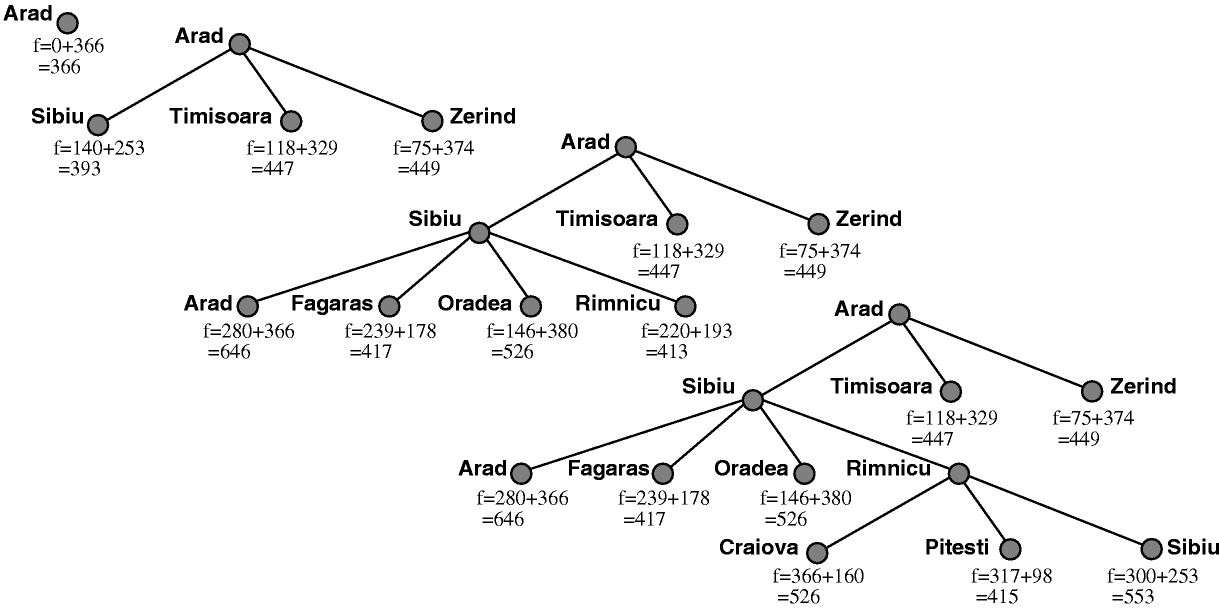
\includegraphics[width=1\textwidth, keepaspectratio]{imgs/searchtree.png}
\end{figure}
\noindent
Search trees are a very useful concept, but as an abstraction. We do \textit{not} want algorithms to store whole search trees as that would require exponential space. We should also discard any nodes in the search tree that are already explored. Search algorithms only store the \textit{frontier} of the search, that is the set of all lead nodes available for expansion at any given point.
\n
We must also be careful of \textbf{loops} in a search tree, where a child node in the tree is the same state as a previous node. Loops can cause certain algorithms to fail, making otherwise solvable problems unsolvable. Usually, there is no need to consider such loops as path costs are additive and step costs are non-negative. A loop to any given state is never better than the same path with the loop removed. Loops are a special case of the more general concept of \textbf{redundant paths}, which are simply heuristically worse off paths than the optimal. In some cases redundant paths are unavoidable. The way to avoid them is to remember where one has been and augment the search algorithm with a list of explored nodes. Newly generated nodes that match previously visited nodes can be discarded. This is known as a \textbf{Graph search} in comparison to a normal tree search.
\subsection{Measuring the performance of search algorithms}
We can evaluate an algorithm's performance in four ways:
\begin{enumerate}
\item \textbf{Completeness}: Is the algorithm guaranteed to find a solution when there is one?
\item \textbf{Optimality}: Does the strategy find the optimal solution?
\item \textbf{Time complexity}: How long does it take to find a solution?
\item \textbf{Space complexity}: How much memory is needed to perform the search?
\end{enumerate}
\noindent
The time and space complexity are always considered with respect to some measure of the problem size or difficulty. As such the complexity is expressed in terms of three quantities:
\begin{enumerate}
\item \textbf{b, the branching factor} - the maximum number of children of any node
\item \textbf{d, the depth} - the shallowest goal node (the least number of steps along the path from the root)
\item \textbf{m, maximum length} - the maximum length of any  path in the search space
\end{enumerate}
\noindent
Time is often measured in terms of the number of nodes generated during the search, and space in terms of the maximum number of nodes stored in memory. The \textbf{search cost} is the cost taken by the algorithm to find the solution, but there is also the \textbf{solution cost}, which is the length of the path, or for example moves made in a board game. 

\subsection{Complete search algorithms}

\subsubsection{Breadth-first search}
\textbf{Breadth-first search} is a simple strategy where the root node is expanded first, then all the children of the root node are expanded next, then their children and so on. In general, all nodes of the current depth are expanded before moving on to the next depth. 
\begin{figure}[H]
\centering
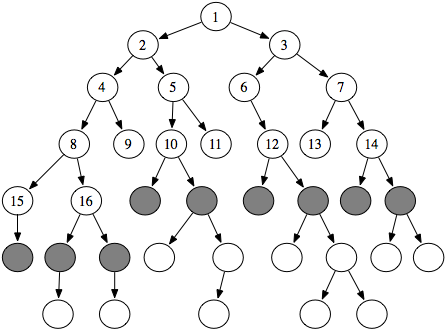
\includegraphics[width=1\textwidth, keepaspectratio]{imgs/breadth-first-search.png}
\end{figure}
\noindent
Implementation of the breadth-first search is very simple using a FIFO queue. Expanded nodes are put at the back of the queue, so all nodes of the same depth are expanded first before the next depth. The problem is that this list can be exponential in size as it contains all nodes at a given depth. We can also use a heuristic to decide what order to add the new states.
\n
There are two major problems with breadth-first search. First, the \textit{memory requirements} are a bigger problem than is the \textit{execution time}. However, time is still a major factor as well. In general, \textit{exponential-complexity search problems cannot be solved by uninformed methods for any but the smallest instances}.
\subsubsection{Depth-first search}
In a \textbf{depth-first} search, always expand the \textit{deepest} node in the current frontier of the search tree. Unlike breadth-first search, we can treat the list as a stack instead of a queue. So new search nodes are put at the \textit{front} of the list. Again we may need a heuristic to decide what order to push new nodes to the stack is. New states will always be in front of all old states in the list.
\begin{figure}[H]
\centering
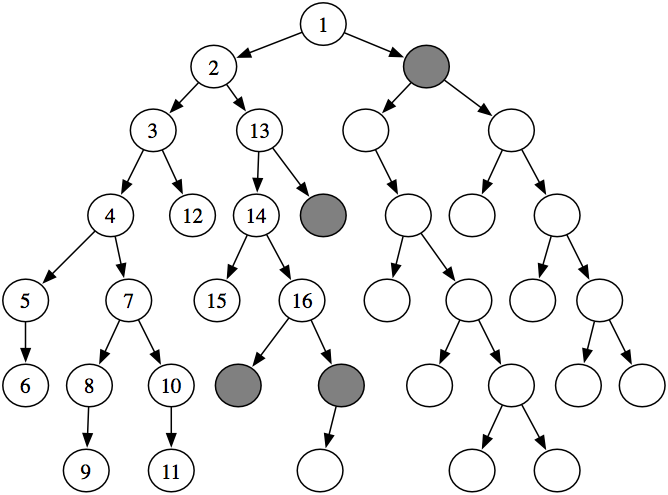
\includegraphics[width=1\textwidth, keepaspectratio]{imgs/depth-first-search.png}
\end{figure}
\noindent
Depth-first search is also non-optimal as it will always search the left subtree first. This means if the solution is somewhere on the right, the search will take longer as it has to go through everything on the left first. Furthermore, if it finds a valid solution, it will return. This may miss out more optimal solutions as it returns after finding the first one. The advantage of depth-first search over breadth-first search is the space complexity. A depth-first search needs to store only a single path from the root to a leaf node, along with any unexpanded sibling nodes for each node on the path. Once a node has been expanded, it can be removed from memory as soon as all its descendants have been fully explored.
\n
The depth of the search is still a problem for depth-first search. If we do not know the depth the solution is found at, the time could take very long to find the solution. If the problem we are trying to solve has an unknown depth, we could go very deep into the tree. This also means we are going very deep down one path of the three before exploring other paths.
\subsubsection{Depth-first depth-bounded search}
A variant on depth-first search, \textbf{depth-first depth-bounded} search limits the depth that the search can go to. This prevents us from going too deep without exploring other branches and also limits the time complexity of the search. However, because it is depth-bounded, the search is not complete as we may search all nodes up to the depth limit without finding the solution. The way to expand and all child nodes is the same as depth-first search, only we do not expand the child nodes once we reach the depth limit. 
\n
Compared to normal depth-first, depth-first depth-bounded will never go down an infinite branch and always find a solution at depth <= the limit. Sometimes, depth limits can be based on knowledge of the problem, or example we know we can mate in three moves. But if we don't know what depth to choose, what should we do then?
\subsubsection{Iterative deepening search}
\textbf{Iterative deepening} is a variant of depth-first depth-bounded where we increase the depth limit on every iteration. This ensures completeness as the search will eventually terminate once it finds a solution at a sufficient depth. However, this search does lots of redundant work as it \textbf{re-evaluates} on \textit{every} iteration, so the first few depths are re-evaluated again and again on every iteration.
\begin{figure}[H]
\centering
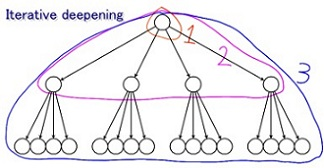
\includegraphics[width=1\textwidth, keepaspectratio]{imgs/iterative-deepening.jpg} 
\end{figure}
\noindent
This may seem very wasteful because states are generated multiple times. It turns out this is not too costly. The reason is that in a search tree with the same branching factor at each level, most of the nodes are in the bottom level, so it does not matter much that the upper levels are generated multiple times. The nodes at the bottom (or rather, the depth where the solution exists) is only generated once, the level above twice and so on. This gives the time complexity as asymptotically the same as breadth-first search. In general, \textit{iterative deepening is the preferred uninformed search method when the search space is large and the depth of the solution is not known.}

\subsubsection{Comparison of search algorithms}

\begin{tabularx}{\textwidth}{|X|XXXX|}
\hline
Criterion & Breadth-first & Depth-first & Depth-first depth-bounded & Iterative deepening \\
\hline
Complete? & Yes & No & No & Yes \\
Time & $O(b^{d})$ & $O(b^{d})$ & $O(b^{d})$ & $O(b^{d})$ \\
Space & $O(b^{d})$ & $O(bd)$ & $O(bd)$ & $O(bd)$ \\
\hline
\end{tabularx}

\subsection{Heuristic search strategies}
\subsubsection{Best-first search}
The idea is to explore the frontier heuristically instead of in a purely algorithmic way. \textbf{Best-first} search is an algorithm in which a node is selected for expansion based on an \textbf{evaluation function} $f(n)$. New states can be sorted in order of the score of that state from the evaluation function. The list always contains the most promising state first. The actual search itself can use the search algorithms from before, like depth-first or iterative deepening. Most best-first algorithms include as a component of $f$ a \textbf{heuristic function} $h(n)$.
\n
$h(n)$ = estimated cost of the cheapest path from the state at node $n$ to a goal state. In this case, if $n$ is a goal node, then $h(n) = 0$.
\n
A \textbf{greedy best-first search} algorithm will always try to expand the node that is closest to the goal. It evaluates nodes by using just the heuristic function, that is $f(n) = h(n)$.  Greedy best-first can be incomplete if we don't keep track of which nodes we have visited before. 

\subsubsection{A* search}
A widely known and popular search algorithm is the \textbf{A* search}. The evaluation function $f(n)$ that it uses is the combination of:
\begin{itemize}
\item $g(n)$ - the cost to reach the node
\item $h(n)$ - the cost to get from the node to the goal state
\end{itemize} 
This gives $f(n) = g(n) + h(n)$. Since $g(n)$ gives the path cost from the start node to node $n$ and $h(n)$ is the estimated cost from node $n$ to the goal, $f(n) = $ estimated cost of the cheapest solution through $n$. Provided that the heuristic function $h(n)$ is an \textbf{admissible} and \textbf{consistent} heuristic, A* search is both optimal and complete.
\begin{figure}[H]
\centering
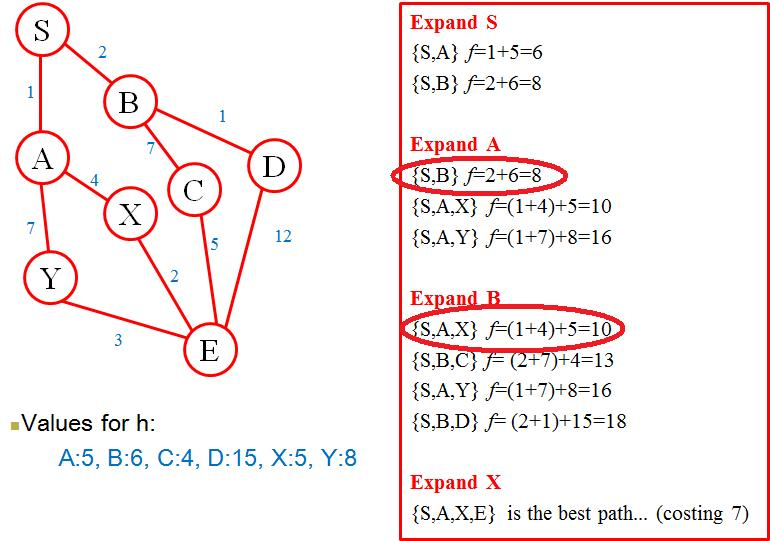
\includegraphics[width=1\textwidth, keepaspectratio]{imgs/a-star.jpg}
\end{figure}
\noindent
For optimality, it is required that the heuristic $h(n)$ is an \textbf{admissible heuristic}. An admissible heuristic is one that \textit{never overestimates} the cost to reach the goal. Typically admissible heuristics think the cost of solving the problem is less than it actually is. For example, an admissible heuristic for calculating distances is the straight-line distance (as the crow flies) from one location to another. It is admissible because the shortest path between any two points is a straight line, so the heuristic cannot be an overestimate.
\n
A second, stronger condition is called \textbf{consistency}. A heuristic $h(n)$ is consistent if, for every node $n$ and every successor $n^{\prime}$ of $n$ generated, the estimated cost of reaching the goal from $n$ is no greater than the step cost of getting to $n^{\prime}$ + the estimated cost of reaching the goal from $n^{\prime}$. In other words:
\begin{equation}
h(n) \leq cost(n^{\prime}) + h(n^{\prime})
\end{equation}
A* \textbf{guarantees} to find the optimal solution.
\n
The problem with A* is that the number of states within the goal search space is still exponential in the length of the solution. There may also be cases in search where we do not need to find the optimal solution and instead prefer to find any solution in less time and space. 
\subsubsection{Branch and Bound}
The \textbf{Branch and bound} algorithm is usually used where there is a natural cost of each node (for example the length of the path). Like A*, it exploits bounds to reduce the amount of search needed, but unlike A*, we can search however we want (i.e, use other search algorithms like depth-first or breadth-first as we please). Usually we search depth-first.
\n
Just like A*, we look for a \textbf{bound} which is guaranteed lower than the true cost. Unlike A*, we are not guaranteed an optimal solution for the first solution found. However, with the bound we can continue search until we find the optimal solution. If the heuristic used is cost + bound and the search used is best-first, the branch and bound \textit{is} A*. 
\begin{figure}[H]
\centering
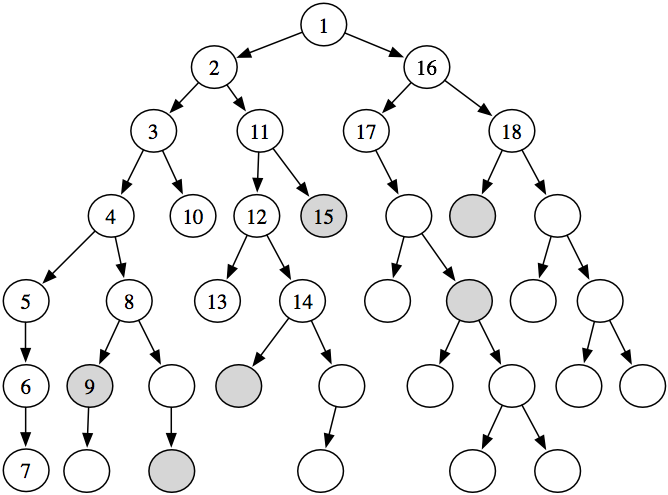
\includegraphics[width=1\textwidth, keepaspectratio]{imgs/branch-and-bound.png}
\end{figure}
\noindent
We add a variable \texttt{best = \infty} which is the score of the best solution so far. It is \infty initially because we don't know if any solution at all is possible. Next, we search according to whatever search method we choose, however:
\begin{itemize}
\item At any node $n$, cut off the search if $f(n) \geq $ \texttt{best}
\item When a solution is found at node $n$, set \texttt{best} $ = g(n)$
\end{itemize}
The idea is we stop searching any deeper if the evaluated score of the node is worse than the currently found best solution. This reduces the amount of search and we are guaranteed to find the best solution because the best solution is one with the minimum \texttt{best} score.
\n
We use branch and bound as A* can be infeasible in practice due to its exponential search space requirement. If we use depth-first as our branch and bound search algorithm, we only need a linear amount and search space and we are still able to exploit heuristics and bounds to find the optimal solution. 

\subsection{Incomplete Search}
The complete search methods we previously looked at all have a key problem, they do \textit{exhaustive} searches on the search space to find the optimal solution. This makes the search very expensive, even with cut-offs like in branch and bound. If there is no solution, these algorithms must do a complete sweep of the search space to verify that. It also means it's hard to jump around the search space even if the algorithm is working in a very unpromising part of it. 
\n
Additionally, in some cases of search problems, the path to the solution doesn't matter, that is the path to the solution is \textit{not} a part of the solution. In cases where the path does not matter, we consider a different class of \textbf{local search} algorithms. Local search algorithms are not systematic in the way they search and operate using a single current node and generally move only to neighbours of that node. There are two key advantages to these algorithms:
\begin{enumerate}
\item They use very little memory - usually a constant amount
\item They can often find reasonable solutions in large or infinite state spaces where systematic (complete) search algorithms are unsuitable
\end{enumerate}
These \textbf{incomplete} search methods don't have to be exhaustive and they exploit this by moving around the search space much more rapidly. The risk is missing solutions that are near where they have just been because they are jumping around. Incomplete search methods typically involve three things:
\begin{enumerate}
\item A representation of a complete search state
\item Some form of \textit{hill climbing} to move towards nearby solutions
\item Some means of making \textit{bad} moves to jump to a different part of the search space
\end{enumerate}
Complete and incomplete search methods are the opposite of each other. Complete methods always have a \textit{consistent} but \textit{partial (incomplete)} search state and are trying to get a \textit{complete} search state. On the other hand, incomplete methods always have a \textit{complete} but \textit{inconsistent} search space and are trying to get a \textit{consistent} search state.
\subsubsection{Hill-climbing search}
The \textbf{hill-climbing} search algorithm is a simple algorithm that continues to try and move in the direction of increasing value (uphill). Given a start state S, it explores all of its neighbours and chooses the highest neighbour (or random if there is a tie). The algorithm does not maintain a search tree and does not need to look ahead beyond the immediate neighbours of the current node. Hill climbing is also called \textbf{greedy local search} because it always goes for the next best neighbour state without thinking ahead about where to go next.
\begin{figure}[H]
\centering
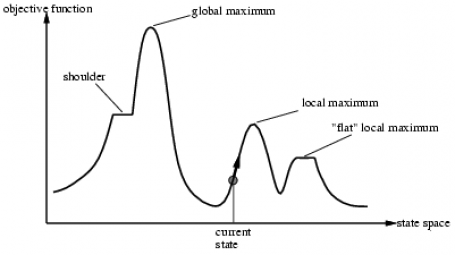
\includegraphics[width=1\textwidth, keepaspectratio]{imgs/hill-climbing.png}
\end{figure}
\noindent
The issue is that the algorithm can get stuck for many reasons:
\begin{itemize}
\item \textbf{Local maxima}: a local maximum is a peak that is higher than each of its neighbouring states, but lower than the global maximum. Hill-climbing algorithms that come near the local maximum will go up to its peak but will then be stuck with nowhere else to go. It does not know to go for a neighbour with less value to try and find a better maximum. 
\item \textbf{Ridges}: A ridge is a sequence of local maxima that is very difficult for greedy algorithms to navigate.
\item \textbf{Plateaux}: A plateau is a flat area, it can either be a ``flat" local maximum, or a \textbf{shoulder} where progress is still possible. Instead of halting the algorithm if it reaches a plateau, it might be a good idea to allow a sideways move in the hop that the plateau is really a shoulder. This raises the percentage of problem instances solved by hill climbing, but comes at a cost of the algorithm taking an average of more steps for each success and failure.
\end{itemize}
Hill climbing algorithms are therefore \textit{incomplete} because of this tendency to get stuck in local maxima. \textbf{Random-restart} is a hill climbing variant that conducts a series of hill climbing searches from randomly generated initial states until the global maximum is found. If each hill climbing search has a probability $p$ of success, then the expected number of restarts required is 1/$p$.
\subsubsection{WalkSAT}
We can combine a random walk where we choose neighbours at random with hill climbing for a better incomplete algorithm. One such example is the \textbf{WalkSAT} algorithm. WalkSAT only applies to the boolean satisfiability problem seen earlier, but it uses concepts of both hill climbing and random walk. 
\begin{lstlisting}[caption={WalkSAT algorithm}, label=algo:walksat]
Choose a random complete truth assignment T
while (T leaves at least one unsatisfied clause) {
	choose an unsatisfied clause C at random
	generate a random number r between 0 and 1
	if (r > p) {
		select variable v in C to flip which maximises the number of satisfied clauses
	}
	else {
		select variable v in C randomly
	}
	Set T = [T with v set to the opposite value]
}
return T
\end{lstlisting}
\noindent
Line 6 is the hill climbing portion of the algorithm and line 9 gives the ``bad" moves portion for random walking. WalkSAT is very effective at local search in SAT, however, it is used less than complete solvers like DPLL because most people want a complete search instead.

\subsubsection{Hill-climbing variants}
There are many hill climbing variants that try to get around the problem of being stuck at local maxima or at plateaus:
\begin{itemize}
\item \textbf{Allow sideways moves} - We have already looked at allowing sideways moves to try and get off a plateau without looping. Most notably, we should only allow $n$ sideways moves so an infinite loop does not occur whenever the algorithm reaches a flat local maximum that is not a shoulder.
\item \textbf{Stochastic hill climbing} - This method chooses at random from among the uphill moves with the probability of selection varying based on the steepness of the uphill move. This usually converges more slowly as it doesn't always choose the steepest (best) move, but it finds better solutions.
\item \textbf{First choice hill climbing} - This implements stochastic hill climbing by generating successors randomly until one is generated that is better than the current state. This is a good strategy when a state has many (i.e, thousands) of successors.
\item \textbf{Random restart} - We have also looked at this before as it is a variant that conducts a series of hill climbs and only stops when the goal is reached. The success of this variant depends very much on the shape and landscape of the space. If there are few local maxima and plateaux, random-restart hill climbing will find a good solution very quickly. However, it is more difficult with more complicated landscapes. Despite this, reasonably good local maximum can often be found after a small number of restarts. This does not give the optimal solution, but often we are do looking for the optimal solution. 
\end{itemize}
\subsubsection{Simulated annealing}
\textbf{Simulated annealing} is a combination of random walk and hill climbing. Instead of using uphill climbing, we switch our point of view to \textbf{gradient descent} where the goal is to minimise the cost. Imagine the situation being trying to roll a ball down a hill, but it could stop at a local minimum. The trick is to shake the surface to try and bounce the ball out of the local minima and keep is rolling. The simulate-annealing solution is to start by shaking hard, and then gradually reduced the intensity of the shaking.
\begin{figure}[H]
\centering
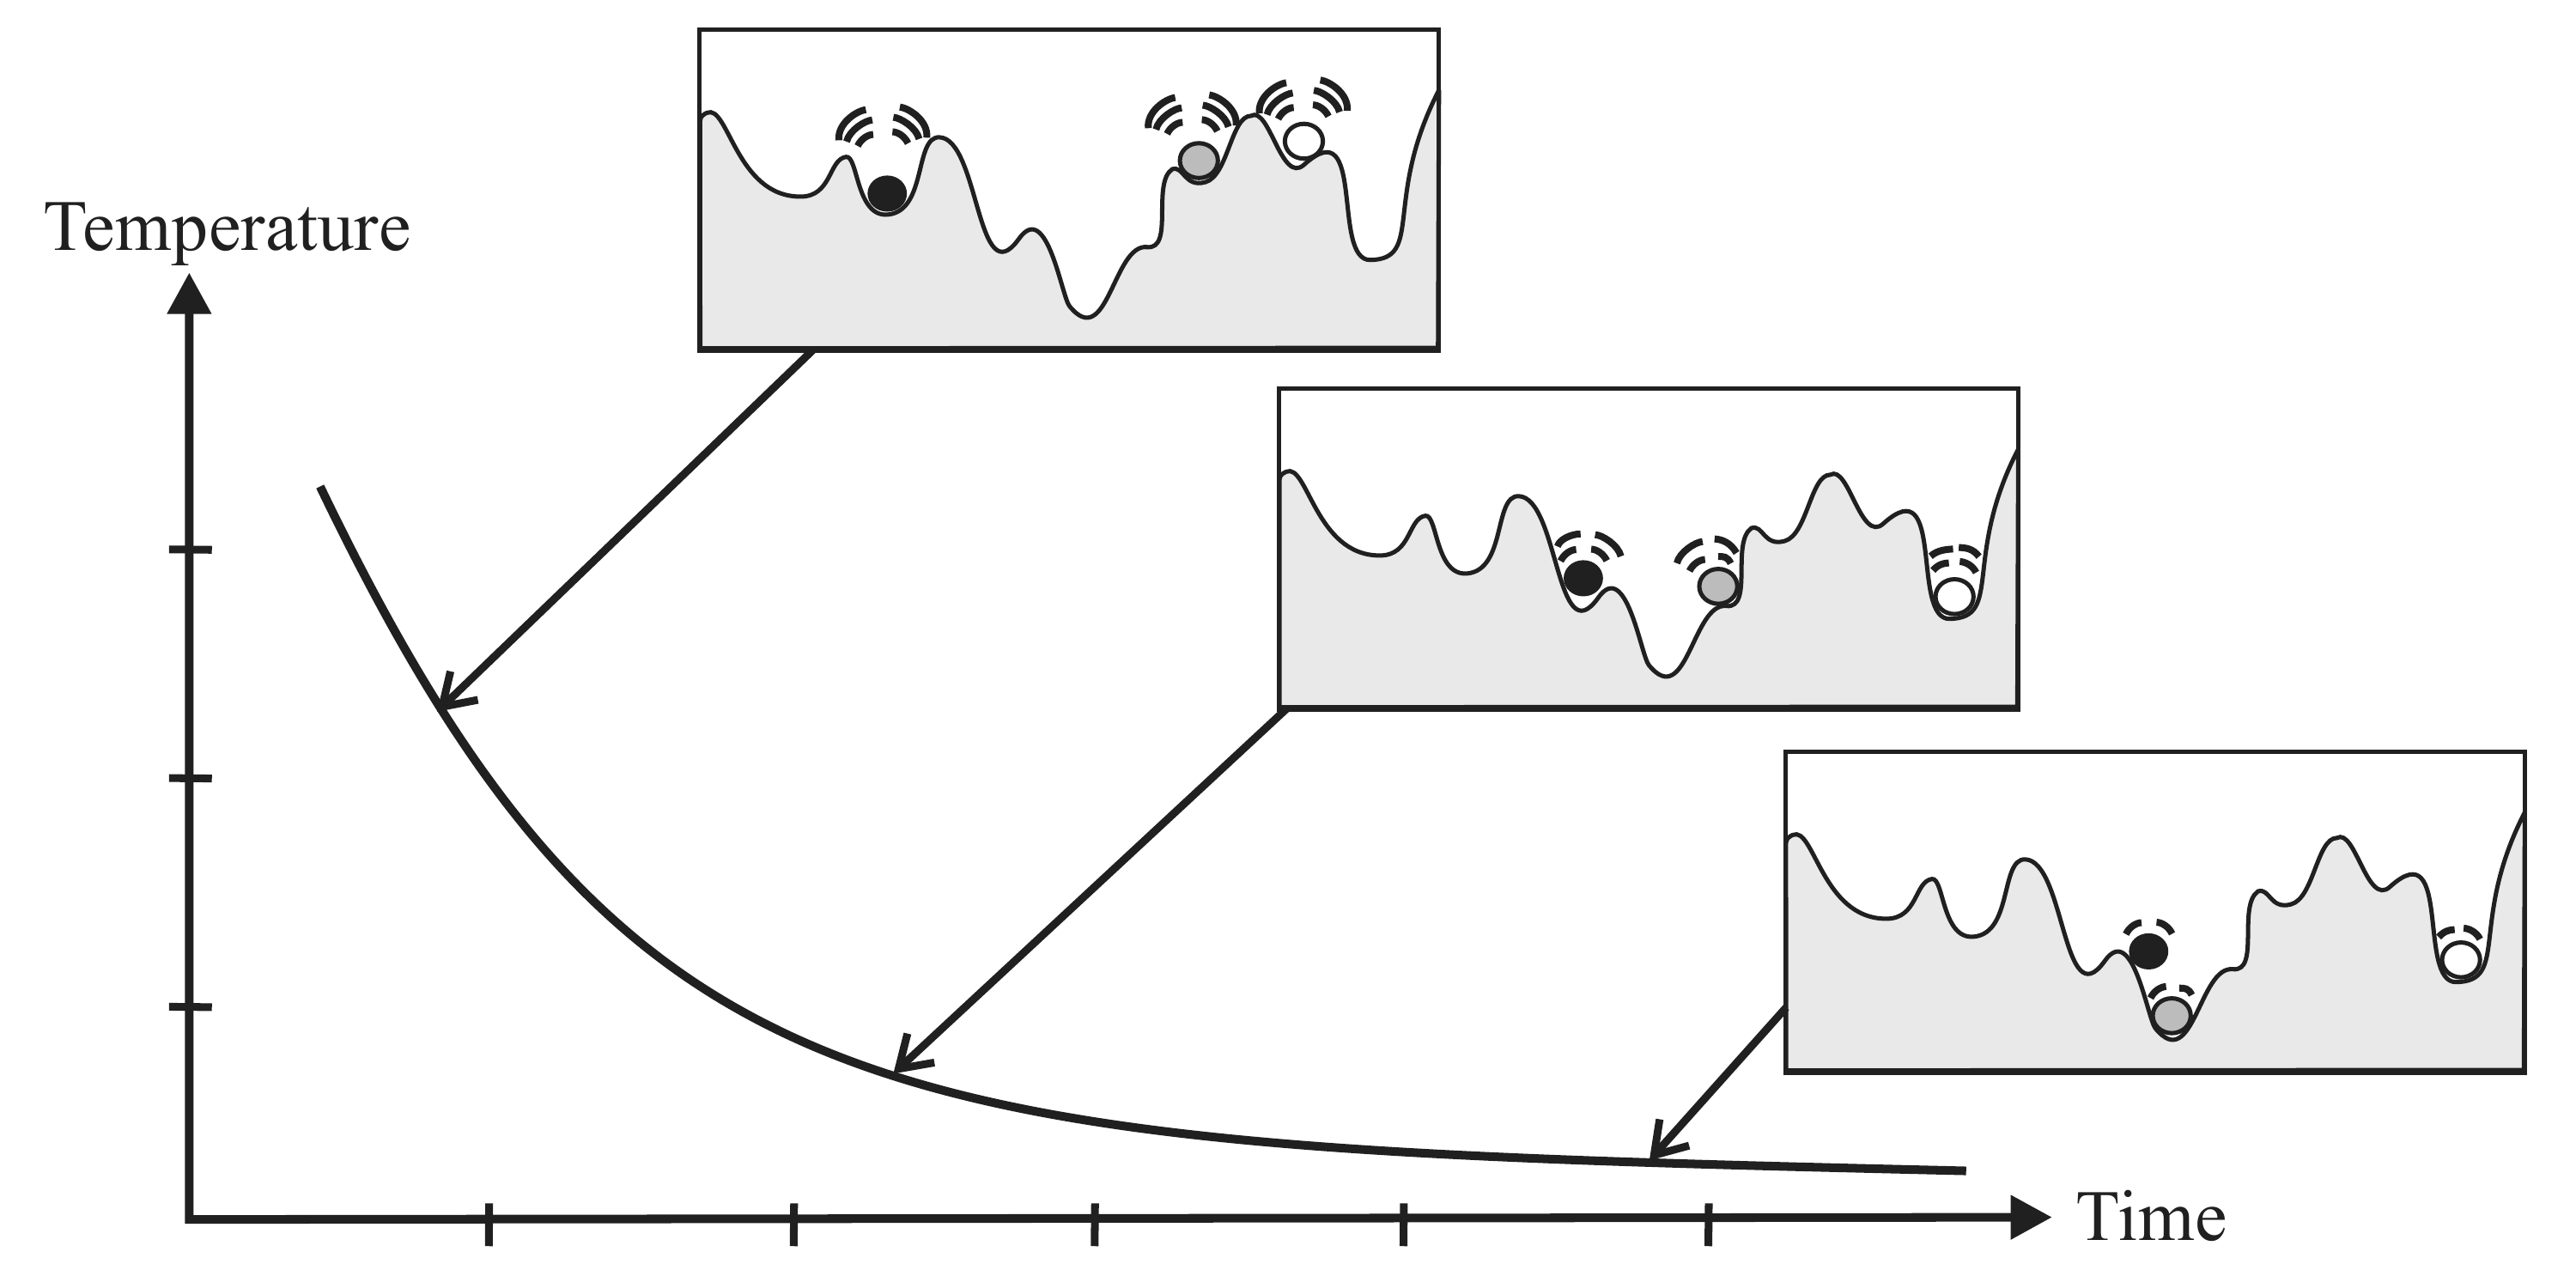
\includegraphics[width=1\textwidth, keepaspectratio]{imgs/simulated-annealing.jpeg}
\end{figure}
\noindent
Instead of picking the \textit{best} move, it picks a \textit{random} move. If the move improves the situation, it is always accepted. Otherwise, the algorithm accepts with some probability $p < 1$. This probability decreases exponentially with the ``badness" of the move. The probability also decreases as the ``temperature" goes down. Therefore bad moves are more likely to be allowed at the start and less as we head towards a solution. If the schedule lowers $p$ slowly enough, then a global optimum will be found with probability of 1.

\subsubsection{Local beam search}
Instead of just keeping one node in memory as hill climbing does, \textbf{local beam search} keeps track of $k$ states. It begins with $k$ randomly generated states. At each step, all the neighbours of all $k$ states are generated. If any of them is the goal then stop, otherwise selected the $k$ best nodes from all the neighbours and repeat.
\n
At first, this just seems like running $k$ random restarts in parallel. However, the two algorithms are quite different. In random-restart, each search process runs independently of the others. In local-beam search, useful information is passed among the parallel search threads. The algorithm quickly abandons unfruitful searches and moves its resources to where the most progress is being made.
\n
In the most simple version of this algorithm, the search can quickly suffer from a lack of diversity among the $k$ states as they can converge to a small region of the search space. A variant called \textbf{stochastic local beam search} helps this problem. Instead of choosing $k$ best nodes from the pool, it chooses the $k$ nodes at random with probability being an increasing function of its value. This is analogous to the process of natural selection. 

\subsubsection{Genetic algorithms}
A \textbf{genetic algorithm} is a variant of stochastic beam search in which two parent nodes are combined to generate the child nodes. This is again an analogy to natural selection, except we have sexual rather than asexual reproduction. Like a beam search, GAs start with $k$ randomly generated states, called the \textbf{population}. Each node is encoded as a string, most commonly of 0s and 1s. 
\begin{figure}[H]
\centering
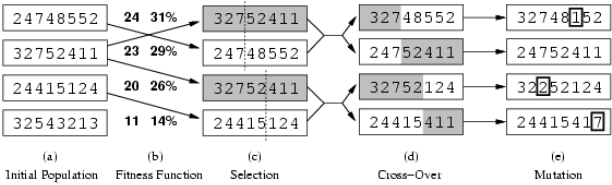
\includegraphics[width=1\textwidth, keepaspectratio]{imgs/genetic-algorithm.png}
\end{figure}
\noindent
The production of the next generation of states is as follows:
\begin{enumerate}
\item Each state is rated by a \textbf{fitness function}, with probability $P($node chosen$) \propto $ node fitness, possibly culling all nodes below a set fitness
\item Next, selection nodes to combine based on the probability $p$ so that less fit nodes are rarely chosen. Note than the same node could be chosen multiple times and some nodes could be not chosen at all.
\item For each pair, a \textbf{crossover} point is chosen randomly from the positions in the strings
\item The offspring are created by crossing over the parent strings at the crosspoint point. This creates two children, though we could discard one and only create one child.
\item Finally, each location of the string is subject to random \textbf{mutation} with a small independent probability. 
\end{enumerate}
New generations and continually produced from the previous generations until some individual is fit enough, or a bound has been reached in terms of number of generations or time. 
\n
Early on, the algorithm makes larger steps as there is a wide divergence of child nodes of the population. But as more generations pass, the steps become smaller as we get closer to the goal as the parent nodes all share many features. The crossover of GAs make it different from local beam search, however it requires very careful design. Some encoding/crossover schemes give no advantages whereas others swiftly raise search granularity. Genetic algorithms work best when the schemata correspond to meaningful components of a solution.
\section{Machine Learning}
An agent is \textbf{learning} if it improves its performance on future tasks after making observations about the world. The first question one might ask is why would we want an agent to learn? If we could improve the design of the agent, surely the designers could just program in the improvements. There are three main reasons why we want agents to learn:
\begin{enumerate}
\item The designers cannot anticipate all possible situations that the agent might find itself in. For example a robot to navigate a maze must learn the layout of each new maze it encounters.
\item The designers cannot anticipate all changes over time. A program designed to predict the weather must adapt to the time of year or location.
\item Sometimes human programmers have no idea how to program the solution themselves. For example, how do we code/program a computer to recognise faces of people?
\end{enumerate}
There are also several components of an agent that can be improved by learning from data. The improvements and the techniques used to make them depend on four major factors:
\begin{enumerate}
\item Which \textit{component} is to be improved?
\item What \textit{prior knowledge} the agent already has
\item What \textit{representation} is used for the data and the component
\item What \textit{feedback} is available to learn from.
\end{enumerate}
Additionally, there are a number of components that these agents have which include:
\begin{itemize}
\item A direct mapping from conditions on the current state to actions, in other words \textit{What action to take under certain conditions}.
\item A means to infer relevant properties of the world from the percept sequence that might be useful
\item Information about the way the world evolves and about the results of possible actions the agent can take, so \textit{how the world is affected by your actions}
\item Utility information indicating the desirability of world states, how something is assessed along some metric.
\item Action-value information indicating the desirability of actions
\item Goals that describe classes of states whose achievement maximizes the agent's utility.
\end{itemize}
A key issue in machine learning is \textit{representation}. We can't just go wild and learn anything. We usually already decided on the representation and we want to learn the values to put into that representation. For example learning to curve fit where we have decided on a polynomial and want to learn the coefficients. Or in a neural net where we have decided the number of layers/neurons and want to learn the weights and thresholds. 
\subsection{Forms of learning}
There are four different ways that machine learning algorithms can get feedback: \textbf{Supervised} learning, \textbf{Reinforcement} learning, \textbf{Unsupervised} learning and \textbf{Semi-supervised} learning.

\subsubsection{Reinforcement learning}
In \textbf{reinforcement learning}, the agent learns from a series of reinforcements - rewards or punishments. The learner is given a sequence of examples, but is not given the right answer for each one. Instead there is a \textit{reward} or \textit{punishment} if the learner gets the answer right or wrong. The learner than has to figure out how to behave to increase rewards in the future. For example, after playing games of chess against other agents, it is rewarded if it wins and punished if it loses. It is then up to the agent to decide which of the actions prior to the reinforcement were most responsible for it. 
\n
This is quite different from supervised learning as the agent is not told what the correct answer is. After a lot of moves in the game, it is told if it won or lost and reinforced accordingly. 

\subsubsection{Unsupervised learning}
In \textbf{unsupervised learning}, the agent learns patterns in the input even though no explicit feedback is given. It is given a bunch of data but with no answers. Typically this is used statistically and the learning task is to \textbf{cluster}: detecting potentially useful clusters of input examples. For example, a taxi company learner might learn from weather reports what is a good day for their company or a bad day and manage demand. This can be done without ever being given labelled examples of each by a teacher. 

\subsubsection{Semi-supervised learning}
\textbf{Semi-supervised} learning is just like supervised learning, but the ``teacher" is not reliable for any number of reasons:
\begin{itemize}
\item There is no objective truth
\item The best humans can do is fallible
\item The data is subject to lying - for example pictures of people and their age, some people may have lied about their age
\item The data is subject to misinterpretation - Is that number a 1 or a 7?
\end{itemize}

\subsubsection{Supervised learning}
In supervised learning, we ``teach" the learner two things: A set of example inputs and for each example, the ``right" answer. For example in a game of chess, the board position is an example input, with the right answer being the best move in that position. A more obvious example would be an image of a bus and the right answer being that is or is not a bus. To measure the accuracy of learning, we can give the agent a \textbf{test set} of examples that are distinct from the training set. 
\begin{figure}[H]
\centering
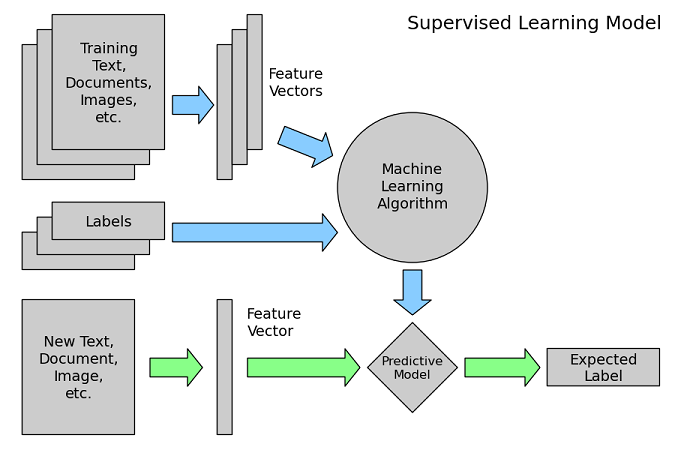
\includegraphics[width=0.8\textwidth, keepaspectratio]{imgs/supervised-learning.png}
\end{figure}
\noindent
When the output $y$ is one of a finite set of values (such as \textit{bus, car, truck}), the learning problem is called \textbf{classification}. If $y$ is a number, the learning problem is called \textbf{regression}. 
\n
The learner has to create a function that gives the correct answer to both new and old (training) inputs. Though this is not always possible, we still want it to give as good an answers as possible. In general, \textit{there is a tradeoff between complex functions that fit the training data well, and simpler functions that may generalise better}.
\begin{figure}[H]
\centering
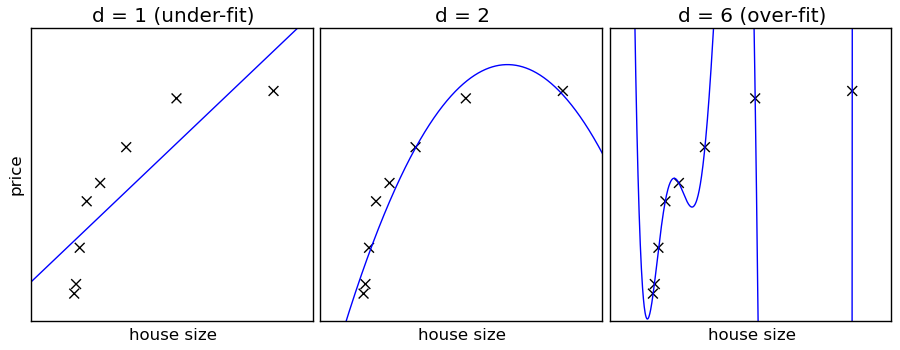
\includegraphics[width=1\textwidth, keepaspectratio]{imgs/supervised-learning-fit.png}
\end{figure}
\noindent
An example problem is curve fitting, where we are trying to find a curve that fits the data points and with this curve, predict $f(x)$ from new inputs of $x$. If we try to fit using a \textbf{linear function} $d = 1$, it is clearly not perfect, but it might be good enough (remember there is a tradeoff between simplicity and accuracy). We could do better with a \textbf{quadratic function} $d = 2$ as it covers most of the points. To us humans this might seem quite a good fit, however we could do \textit{even} better with a function $d = 6$ that fits all the points perfectly. The danger here is of \textbf{overfitting} our data and therefore being unable to generalise. So how do we choose from among multiple consistent functions?
\n
The principle of \textbf{Occam's Razor} is to prefer the \textit{simplest} function that is consistent with the data. Defining simplicity is not easy, but it is clear that a degree-1 polynomial is simpler than a degree-7 polynomial. However, even with Occam's Razor, we still may not know which curve to prefer so we have to choose a tradeoff of simplicity and better fitting the data. 
\n
The term \textbf{Overfitting} means that there is not enough data to justify our git. It is a critical problem in machine learning and especially supervised learning. If we overfit our data, not only do we have a complicated prediction, but it might make nonsense predictions when it comes to new input data. 

\subsection{Decision Trees}
A \textbf{decision tree} represents a function that takes as input a vector of attribute values and returns a ``decision" - a single output value. The input and output values can be discrete or continuous but for now let's focus on the discrete values. 
\n
A decision tree reaches it's decision by performing a sequence of tests. Each internal node in the tree corresponds to a test of the value of one of the input attributes. The branches from the node are labelled with the possible values of the attribute. As a running example, let's decide whether to wait at this restaurant to eat or not to wait. First we list the attributes that we will consider as part of the input:
\begin{enumerate}
\item \textit{Alternate}: is there a suitable alternative restaurant nearby?
\item \textit{Bar}: is the restaurant's bar a comfortable place to wait in?
\item \textit{Fri/Sat}: is it a Friday or Saturday?
\item \textit{Hungry}: are we hungry?
\item \textit{Patrons}: how many people are in the restaurant? (values are \textit{None}, \textit{Some} and \textit{Full}).
\item \textit{Price}: the restaurant's price range (\$, \$\$, \$\$\$)
\item \textit{Raining}: is it raining outside?
\item \textit{Reservation}: do we have a reservation?
\item \textit{Type}: the type of restaurant (French, Italian, Thai or burgers)
\item \textit{WaitEstimate}: the wait estimated by the host (0-10 minutes, 10-30, 30-60 or $>$ 60)
\end{enumerate}
Note that every attribute has a small set of possible values; the value of \textit{WaitEstimate} is not an integer, but one of four discrete values. 
\n
Also to note is that a boolean decision tree is logically equivalent to the assertion that the goal attribute is true if and only if the input attributes satisfy one of the paths leading to a leaf with value \textit{True}. Writing this in propositional logic gives us:
\begin{equation}
Goal \Leftrightarrow (Path_{1} \vee Path_{2} \vee ...)
\end{equation}
Each \textit{Path} is a conjunction of attribute-value tests required to follow that path. Therefore, the whole expression is equivalent to DNF (disjunctive normal form), which means that any function in propositional logic can be expressed as a decision tree. An example path is:
\begin{equation}
Path_{1} = (Patrons == Full \wedge WaitEstimate == 0-10)
\end{equation}
\subsubsection{Supervised learning with decision trees}
An example for a boolean decision tree consists of an ($x$, $y$) pair where $x$ is a vector of values for the input attributes and $y$ is a single boolean output value. Given a set of training examples, we can use an algorithm to build a decision that that could classify new unseen inputs. 
\begin{figure}[H]
\centering
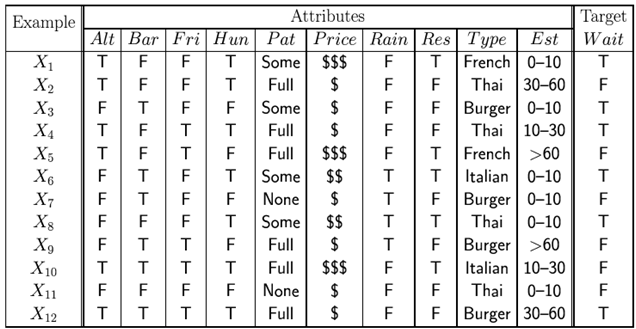
\includegraphics[width=1\textwidth, keepaspectratio]{imgs/decision-tree-table.png}
\end{figure}
\noindent
By Occam's razor, we want a tree that is both consistent with the training examples, but also as small as possible. However there is no efficient way to search through all $2^{2^{n}}$ possible decision trees so we must use some heuristics. With heuristics we can find a small (but not the smallest) consistent tree. The \textbf{decision tree learning} algorithm adopts a greedy divide-and-conquer strategy: \textit{always test the most important attribute first}. The ``most important attribute" means the one that makes the most difference to the classification of the examples. This way, we hope to get the correct classification with a small number of tests, so the paths of the tree are short and the tree as a whole will be shallow.
\begin{figure}[H]
\centering
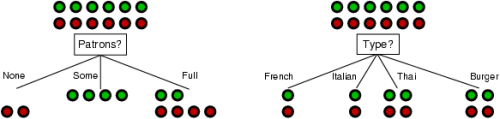
\includegraphics[width=1\textwidth, keepaspectratio]{imgs/decision-tree-split.png}
\end{figure}
\noindent
In our restaurant example, \textit{Type} is a poor attribute to choose first, because it leaves us with four possible outcomes, each of which have the same number of positive and negative examples. On the other hand \textit{Patrons} is an important attribute as the values of \textit{None} and \textit{Some} leave example sets which can immediately be answered definitively. After the first attribute test splits the examples up, each outcome is a new decision tree learning problem in itself, with fewer examples and one less attribute. 
\n
There are four cases to consider for the recursive problems for the sub-problems in the tree:
\begin{enumerate}
\item If the remaining examples are all positive or negative, then we are finished as we can definitively answer \textit{Yes} or \textit{No}. 
\item If there are some mixed positive or negative examples, choose the next best attribute to split them again.
\item If there are no examples left, it means that no example has been observed for this combination of attribute values and we return a default value calculated from the plurality classification of all the examples that were used in constructing the node's parent. 
\item If there are no attribute left, but there are still positive and negative examples, it means these examples have exactly the same description but different classifications. This can occur due to error or noise in the data. The best we can do in this case is return the plurality classifications for the remaining examples.
\end{enumerate}
\begin{lstlisting}[caption={Decision tree learning algorithm}, label=algo:dtl]
function DTL(examples, attributes, default) {
	if (examples is empty) {
		return default
	}
	else if (all examples have the same classification){
		return the classification
	}
	else if (attributes is empty) {
		return PLURALITY(examples)
	}
	else {
		best = CHOOSE_ATTRIBUTE(attributes, examples)
		tree = a new decision tree with root test best
		for each value v of best {
			examples_{i} = {elements of examples with best = v}
			subtree = DTL(examples_{i}, attributes - best, PLURALITY(examples))
			add a branch to tree with label v and subtree subtree
		}
		return tree
	}
}
\end{lstlisting}
The learning algorithm will always construct a decision tree that is consistent with the examples it is given. It should also be considerably small, not having to look at all the attributes to classify all the examples it is given. For cases it has never seen, the algorithm will classify based on the decision tree regardless of whether the actual answer is correct or not. With more training examples, the learning program can correct any mistakes it might make from unseen input.

\subsubsection{Information gain}
A perfect attribute divides the examples into sets where each are all positive or all negative and thus will be leaves of the tree. We can use the notion of information gain, which is defined in terms of \textbf{entropy}.
\n
Entropy is a measure of the uncertainty of a random variable and gain in formation corresponds to a reduction in entropy. The equation for entropy is as follows:
\begin{equation}
H(V) = \sum_{k}P(v_{k})\text{log}_{2}(\frac{1}{P(v_{k})}) = - \sum_{k}P(v_{k})\text{log}_{2}P(v_{k})
\end{equation}
We also define $B(q)$ as the entropy of a Boolean random variable that is true with probability $q$:
\begin{equation}
B(q) = -(q\text{log}_{2}q + (1 - q)\text{log}_{2}(1 - q))
\end{equation}
If a training set contains $p$ positive examples and $n$ negative examples, then the entropy of the goal attribute on the whole set is:
\begin{equation}
H(\text{Goal}) = B\bigg(\frac{p}{p+n}\bigg)
\end{equation}
The \textbf{information gain} from the attribute test on A is the expected reduction in entropy:
\begin{equation}
Gain(A) = B\bigg(\frac{p}{p+n}\bigg) - Remainder(A)
\end{equation}
\begin{equation}
Remainder(A) = \sum_{k=1}^{d}\frac{p_{k} + n_{k}}{p + n}B\bigg(\frac{p}{p+n}\bigg)
\end{equation}
For example, after \textit{Patron}, the information gain is 0.54 bits.
\begin{equation}
Gain(Patron) = 1 - [\frac{2}{12}B(\frac{0}{2}) + \frac{4}{12}B(\frac{4}{4}) + \frac{6}{12}B(\frac{2}{6})] = 0.541\ \text{bits}
\end{equation}
That is:
\begin{itemize}
\item 2/12 chance of gain of 1 bit (\textit{None})
\item 4/12 chance of gain of 1 bit (\textit{Some})
\item 6/12 chance of gain of 0.08 bits (\textit{Full})
\end{itemize}
The attribute with the highest information gain is the one that should be select as the best attribute in the decision tree learning algorithm.
\subsubsection{Learning curve}
We can evaluate the accuracy of a learning algorithm with a \textbf{learning curve}. If we have 100 examples, we can split into a training set and test set. We get a function and then measure its accuracy with the test set. The curve shows that as the training set grows, the accuracy increases.
\begin{figure}[H]
\centering
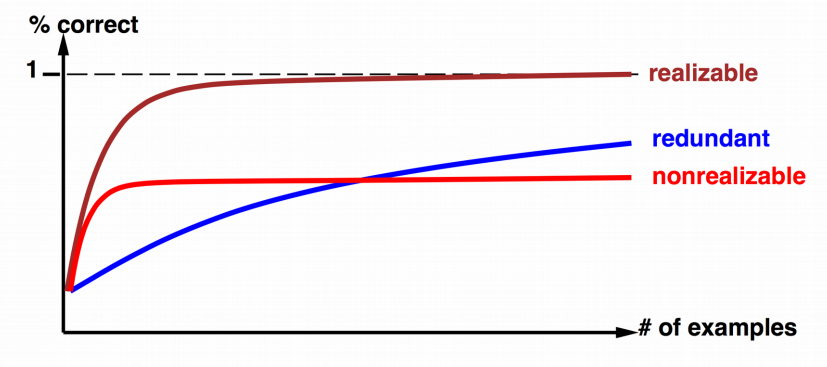
\includegraphics[width=0.9\textwidth, keepaspectratio]{imgs/decision-tree-learning-curve.png}
\end{figure}
\noindent
There are three things we can learning from the learning curve:
\begin{enumerate}
\item \textbf{Realisable} - the representation is able to learn a perfect function in a reasonable number of training examples
\item \textbf{Non-realisable} - the representation is \textit{not} able to learn a perfect function even with infinite examples. For example if the true method is ``toss a coin", we can't get better than 50\% learning
\item \textbf{Redundant} - If there are too many attributes, we might find it hard to tell between similar attributes and other attributes might get lucky on the training set without actually being good.
\end{enumerate}
\subsubsection{Cross validation}
If we don't have limited data, we can do cross validation. The simplest approach is one where we randomly split the available data into training and testing set. This method is called \textbf{Holdout cross-validation}. The disadvantage is that it failed to use all the available data for training. 
\n
A cleverer approach is called \textbf{k-fold cross-validation}. The idea is that each example is used both as training data and test data. First we split the data into $k$ equal subsets. Then we perform $k$ rounds of training. On each round, 1/$k$ of the data is held out as a test set and the remaining examples used as training data. For example if we set $k = 10$. We divide the data into 10 sets and use 9 of the sets for training and 1 for testing. Do this each of the 10 possible ways. The extreme is to have $k = n$, also known as \textbf{leave-one-out cross-validation}. These methods all try to assess how likely our data is to do well against unseen data.

\subsection{Neural networks}

\section{Games playing}
In AI, the most common kind of games are \textbf{zero-sum} or \textbf{perfect information} games. These are games such as chess or go, where both players know everything there is to know about the game position. There is no hidden information and no random events, however the two players need not have the same set of moves available. This means deterministic, fully observable environments where two agents act alternately and the utility values at the end of the game are always equal and opposite. For example if one player wins the game of chess, the other player \textit{must} have lost.
\n
Games are very interesting as often the branching factor is very high, $35^{100}$ for chess so complete search of the game space is not feasible. Even so, an agent must be able to make \textit{some} decision when it is not possible to calculate the \textit{optimal} decision. Games also penalise inefficiency heavily, as we must make use of available time to play.
\n
There are a few techniques that we can use in game playing algorithms. \textbf{Pruning} allows us to ignore portions of the search tree that make no difference to the final choice, or are bad moves that should never be made. Heuristic \textbf{evaluation functions} allow us to approximate the true utility of a game state without doing a complete search. A game can be formally defined as a king of search problem with the following elements:
\begin{itemize}
\item \textsc{$S_{0}$} - The \textbf{initial state} of the game. For example a blank board for Go, or the starting position for Chess.
\item \textsc{PLAYER($s$)} - The player whose turn it is in a given state.
\item \textsc{ACTION($s$)} - The set of legal moves in a given state.
\item \textsc{RESULT($s, a$)} - The \textbf{transition model}, which defines the result of a move on the state.
\item \textsc{TERMINAL-TEST($s$)} - A \textbf{terminal test} to test whether the game is over or not.
\item \textsc{UTILITY($s, p$)} - A \textbf{utility function} which is a numeric value for a game that ends in a terminal state $s$ or a player $p$. Note, this is the \textbf{payoff} and \textit{not} the evaluation function and only applies to terminal states. For example the payoff in Chess would simply be +1 for a win, 0 for a draw and -1 for a loss. In Backgammon, the payoff ranges from 0 to +192 as the score of the game.
\end{itemize}
The initial state, \textsc{ACTIONS} function and \textsc{RESULT} function define a \textbf{game tree} for the game. 
\subsection{Game trees}
A \textbf{game tree} is like a search tree where each node is a search state with full details about the position. The edges between the nodes correspond to moves in the game. The leaf nodes of the tree are determined positions such as win/lose/draw or a certain number of points for or against the player. At each depth, it is one or the other player's turn to make a move.
\begin{figure}[H]
\centering
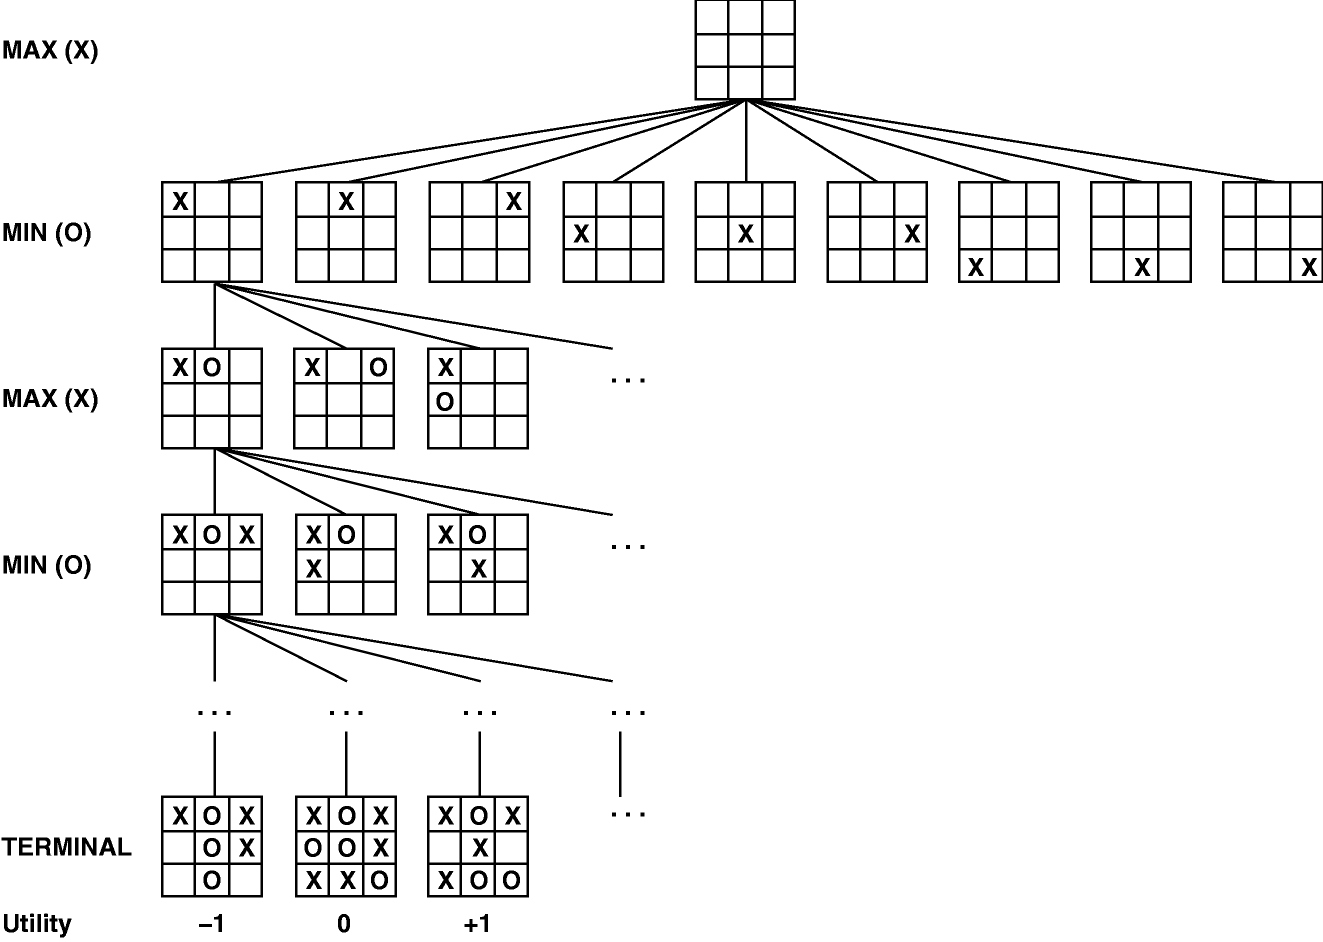
\includegraphics[width=1\textwidth, keepaspectratio]{imgs/gametree.png}
\end{figure}
\noindent
There are strong similarities between search trees and game trees. Infinite loops may also exist in game trees, for example moving a Rook back and forth over and over again. The key difference between a game tree and a search tree is that there is an \textbf{opponent}. Because of this opponent, it is not good enough just to find a path to win a game, the agent must have some form of winning strategy that it uses. We cannot just look at one leaf node and typically need lots of different winning leaf nodes.
\n
Because it is usually impossible to solve games completely and do a complete search of the game tree, we usually can't see any leaf nodes at most points during the game. So we have to \textit{estimate} the cost of internal nodes with a \textbf{static evaluation function} that gives a heuristic value of the node. An evaluation function is an estimate of the true value of a node and can partially indicate the position of the game. An example evaluation function for chess would be having each piece be worth certain values: $Pawn = 1$, $Knight = Bishop = 3$, $Rook = 5$, $Queen = 9$, $King = 1000$.
\subsection{The minimax algorithm}
We consider a game with two players, \textsc{max} and \textsc{min}. \textsc{max} wants to maximise his score while \textsc{min} wants to minimise her score. The optimal strategy can be determined from the \textbf{minimax value} of each node, which is the utility of being in the corresponding state, \textit{assuming that both players play optimally}. Given the choice, \textsc{max} prefers to move to a state with higher value and \textsc{min} prefers a state of lower value. 
\begin{figure}[H]
\centering
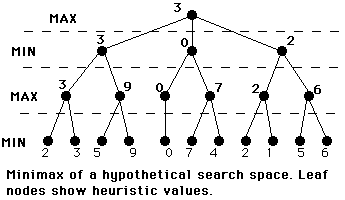
\includegraphics[width=0.8\textwidth, keepaspectratio]{imgs/minimax.png}
\end{figure}
\noindent
The algorithm computes the minimax decision at the current node. Then it simply uses recursion to work out the static evaluations (or minimax decisions) of all child nodes either until the leaf nodes or down until a certain depth. Then all the values are propagated upwards through the tree. The score of the \textsc{max} nodes is the maximum value of its child nodes and vice versa for the \textsc{min} nodes. Propagating all the way back up to the current node (root node) gives the score of possible moves from the root node and hence the best move to make. The algorithm performs a complete depth-first exploration of the game tree, so it is space efficient. 
\n
The problem with the minimax algorithm is that it is \textit{horrendously} inefficient. If we go to a depth $d$ with a branching rate of $b$, then we must explore $b^{d}$ nodes and calculate the score at every node. This is exponential to the depth of the tree. However, much of this work is wasted as we don't need to know the score of those nodes. The trick is to \textbf{prune} the tree to eliminate nodes in the game tree we do not need to explore.
\subsection{Alpha-Beta pruning}
\textbf{Alpha-beta pruning} works by pruning away branches that have no influence on the final decision. It returns the same move as minimax would, except we have to search less of the game tree. Alpha-beta pruning can be applied to trees of any depth and can often prune entire subtrees rather than just leaves.
\n
We have two parameters \alpha\ and \beta\ that describe the bounds on the backed-up values that appear on the nodes of the tree.
\begin{itemize}
\item \alpha\ = the value of the best (highest value) choice we have found so far at any choice point along the path for \textsc{max}.
\item \beta\ = the value of the best (lowest value) choice we have found so far at any choice point along the path for \textsc{min}.
\end{itemize}
Alpha-beta search updates the values of \alpha\ and \beta\ as it goes through the depth first search and prunes any branches at a node as soon as the value of the current node is known to be worse than the current \alpha\ or \beta\ value for \textsc{max} and \textsc{min} respectively. Either a \alpha\ or \beta\ cutoff can occur.
\begin{figure}[H]
\centering
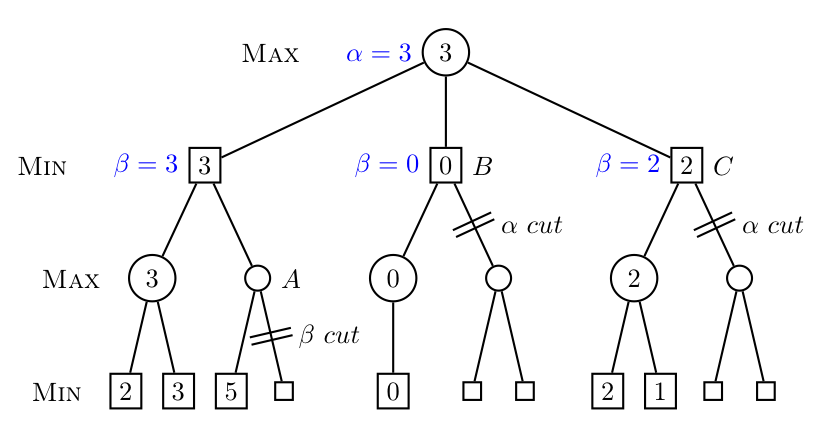
\includegraphics[width=0.9\textwidth, keepaspectratio]{imgs/alphabeta.png}
\end{figure}
\noindent
An \textbf{alpha cutoff} occurs at a \textsc{min} node, when $\alpha \geq \beta$ \\
A \textbf{beta cutoff} occurs at a \textsc{max} node, when $\beta \leq \alpha$
\n
In other words, at every node, check if the \alpha\ value is \geq\ than the \beta\ value, if it is, cut off the search and go back up to the parent node.
\begin{lstlisting}[caption={Alpha-Beta Algorithm}, label=algo:alpha-beta, mathescape=true]
function alphabeta(node, depth, $\alpha$, $\beta$, isMaxNode) {
	if (depth == 0 or node is a leaf node) {
		return heuristic value of node;
	}
	if (isMaxNode) {
		v = -$\infty$;
		for each child in node {
			v = max(v, alphabeta(child, depth-1, $\alpha$, $\beta$, false));
			$\alpha$ = max($\alpha$, v);
			if ($\alpha\ \geq\ \beta$) {
				/* Beta cutoff */
				break;
			}
		return v;
	}
	else {
		v = $\infty$;
		for each child in node {
			v = min(v, alphabeta(child, depth-1, $\alpha$, $\beta$, true));
			$\beta$ = min($\beta$, v);
			if ($\alpha\ \geq\ \beta$) {
				/* Alpha cutoff */
				break;
			}
		return v;
	}
}
\end{lstlisting}
To calculate the \alpha\ and \beta\ values of each node, we get the final backed-up value of its children. As we get the values of each child, we update the current \alpha\ or \beta\ value if it's greater or less than the previous value of a \textsc{max} and \textsc{min} node respectively. Then when we have gone through all the children, we can update the parent node's \alpha\ or \beta\ value. Note when we update the parent, we switch from \alpha\ to \beta\ or vice versa because the parent is the opposite player. As we are going through to get the value of each child, a \textbf{cutoff} can occur at any point. If a cutoff occurs, then the currently stored value of \alpha\ or \beta\ becomes the final backed-up value of this node. 
\subsubsection{Move ordering heuristics}
The effectiveness of alpha-beta pruning is highly dependent on the order in which the states are examined. Depending on the ordering, we could prune entire subtrees, or in a pathological case, we may prune no nodes or very little. This is essentially a question of which child nodes do we expand first?
\n
A \textbf{optimal moves ordering} heuristic for alpha-beta is where we always consider the best moves first. In other words, test the move which has the best final backed-up value first. In practice this is impossible, however with this heuristic, alpha-beta only needs $O(b^{m/2})$ instead of $O(b^m)$. This means that the effective branching factor becomes $\sqrt{b}$ instead of $b$, allowing us to search twice as deep in the same time. With some heuristics such as ordering by a static evaluation that are practical, we can get good performance that is between $\sqrt{b}$ and $b$. 

\subsection{Endgame database}
Sometimes, it might be overkill for game playing AIs to search through millions of search trees just for its opening moves. For example in chess, there have been many books on how to play the opening and endgame. Therefore our computer program can use a \textbf{look-up table} to store a list of good opening moves to play. Statistics on each set of opening moves can also be gathered in a database of previously played games to get a statistically best opening move. This works for the first few moves, though after around 10 moves, the agent must go back to searching as the board position is one that is rarely seen. 
\n
Similarly, in the endgame, there are again few possibilities. For example in chess, only a few pieces remain on each side. Here, a computer can simply store all the millions of combinations of pieces and positions in a database and from that know what the best move is in \textit{any} endgame position. 
\n
To generate endgame databases, there are four steps:
\begin{enumerate}
\item Generate every possible position. For example if there are 2 Knights and a King for B and 1 Knight, 1 Rook, 1 King for W, generate all the possible combinations of positions the pieces can be in. 
\item For each position, mark as a win if W won, marks as a loss if W lost and mark as drawn otherwise.
\item While there are new positions that are marked, for every unmarked position with W to move, mark as win if the move leads to a win and mark as loss if the move leads to a loss. Do the same for B.
\item All unmarked positions are marked as drawn.
\end{enumerate}
Once all the positions are marked, we know the number of moves to win for every position and so knowing the status of any position in the database is just a single lookup. To find the best move in any Win/n position, it is simply any Win/n-1 position. 
\subsection{Monte Carlo Tree Search}
The name \textbf{Monte Carlo} is a general technique in Computer Science and other areas beyond. It is used when one can't sample more than a small percentage of the full search space. Instead we generate \textbf{random} cases and use these to build up a statistical sample of the truth. Instead of searching the tree exhaustively, simply \textit{sample} it. Then play each branch you look to the end of the game, making random moves and add the results as to who wins to the tree. This means we don't need a static evaluation because we know the winner/loser.
\begin{figure}[H]
\centering
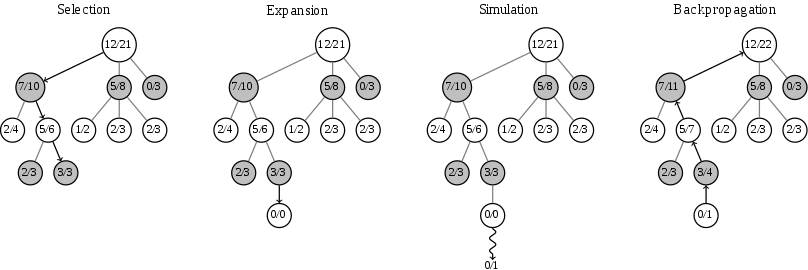
\includegraphics[width=1\textwidth, keepaspectratio]{imgs/mcts.png}
\end{figure}
There are four stages to Monte Carlo Tree Search:
\begin{enumerate}
\item \textbf{Selection} - Select a node to expand using a \textbf{policy}. The policy should have a balance between \textit{exploitation} of known good moves and \textit{exploration} of less visited moves.
\item \textbf{Expansion} - Choose the heuristically ``best" move which has not yet been expanded and expand the selection node. 
\item \textbf{Simulation} - Simulate from this new node to the \textit{end of the game}, usually with random moves
\item \textbf{Back-propagation} - Finally, propagate the results back up the tree and update the statistics of each expanded node to record who won the game. 
\end{enumerate}
The Monte Carlo Tree Search algorithm has many distinct advantages which make it very suitable for games without perfect information or games where the search space and branching rate is too high or it is difficult to come up with a static evaluation function. The problem with MCTS is it can take a long time to converge to accurate assessments of moves, though we can add heuristics to improve this. This is the main method (along with machine learning) that has revolutionised Computer Go playing.
\subsection{Solving checkers}

\section{Automated Reasoning}
\subsection{What is logic?}
Logic is reasoning to deduce new facts given facts we already have and the study of how that reasoning is done. It can be done in any language, but it can also be done using \textit{symbols}. We are mostly concerned with \textbf{symbolic logic}, that is, logical reasoning where we are dealing with symbols. 
\n
Logical sentences must be expressed both according to the \textbf{syntax} and \textbf{semantics}. The notion of syntax is what specifies all the sentences that are well formed. For example in normal arithmetic, the sentence ``$x + y = 4$" follows proper syntax, whereas ``$x4y+=$" does not. Semantics defines the meaning of \textbf{truth} of each sentence with respects to \textit{each possible word}. For example the sentence ``$x + y = 4$" is true in a world where $x = 2$ and $y = 2$ or $x = 3$ and $y = 1$. However, it is false in a world where $x = 1$ and $y = 1$. In standard logics, every sentence must be either true or false, there is no in between.
\n 
There isn't just one kind of symbolic logic, in fact there are \textit{many}. There are two main reasons why there are different kinds of logic:
\begin{enumerate}
\item We might choose one logical system over another for efficiency or where one system is better suited for the given task. This is analogous to having different programming languages, where one might choose the language based on the task. In general, there is a tradeoff between the \textbf{expression power} of that logic system and the \textbf{reasoning complexity} of that logic. The more expressive power a logic has, the more it can express concepts \textit{easily} and \textit{accurately}. Easily here means we can write things down more concisely and accurately means we can write things down which equate to what we really mean. For example \textbf{propositional logic} allows us only to express ``propositions" while \textbf{first order logic} allows us to express facts and relationships between objects.
\item Different logic systems give us \textit{different results}. We might want to reason in different ways in different situations to more accurately depict the situation. Take this sample situation: A shop has two copies of ``Wisden 1976", one hardback and one paperback. Another customer had preordered a copy but the bookseller could not remember which version so he got one of each and is waiting for that customer. The question is can we buy a copy of ``Wisden"?
\begin{figure}[H]
\centering
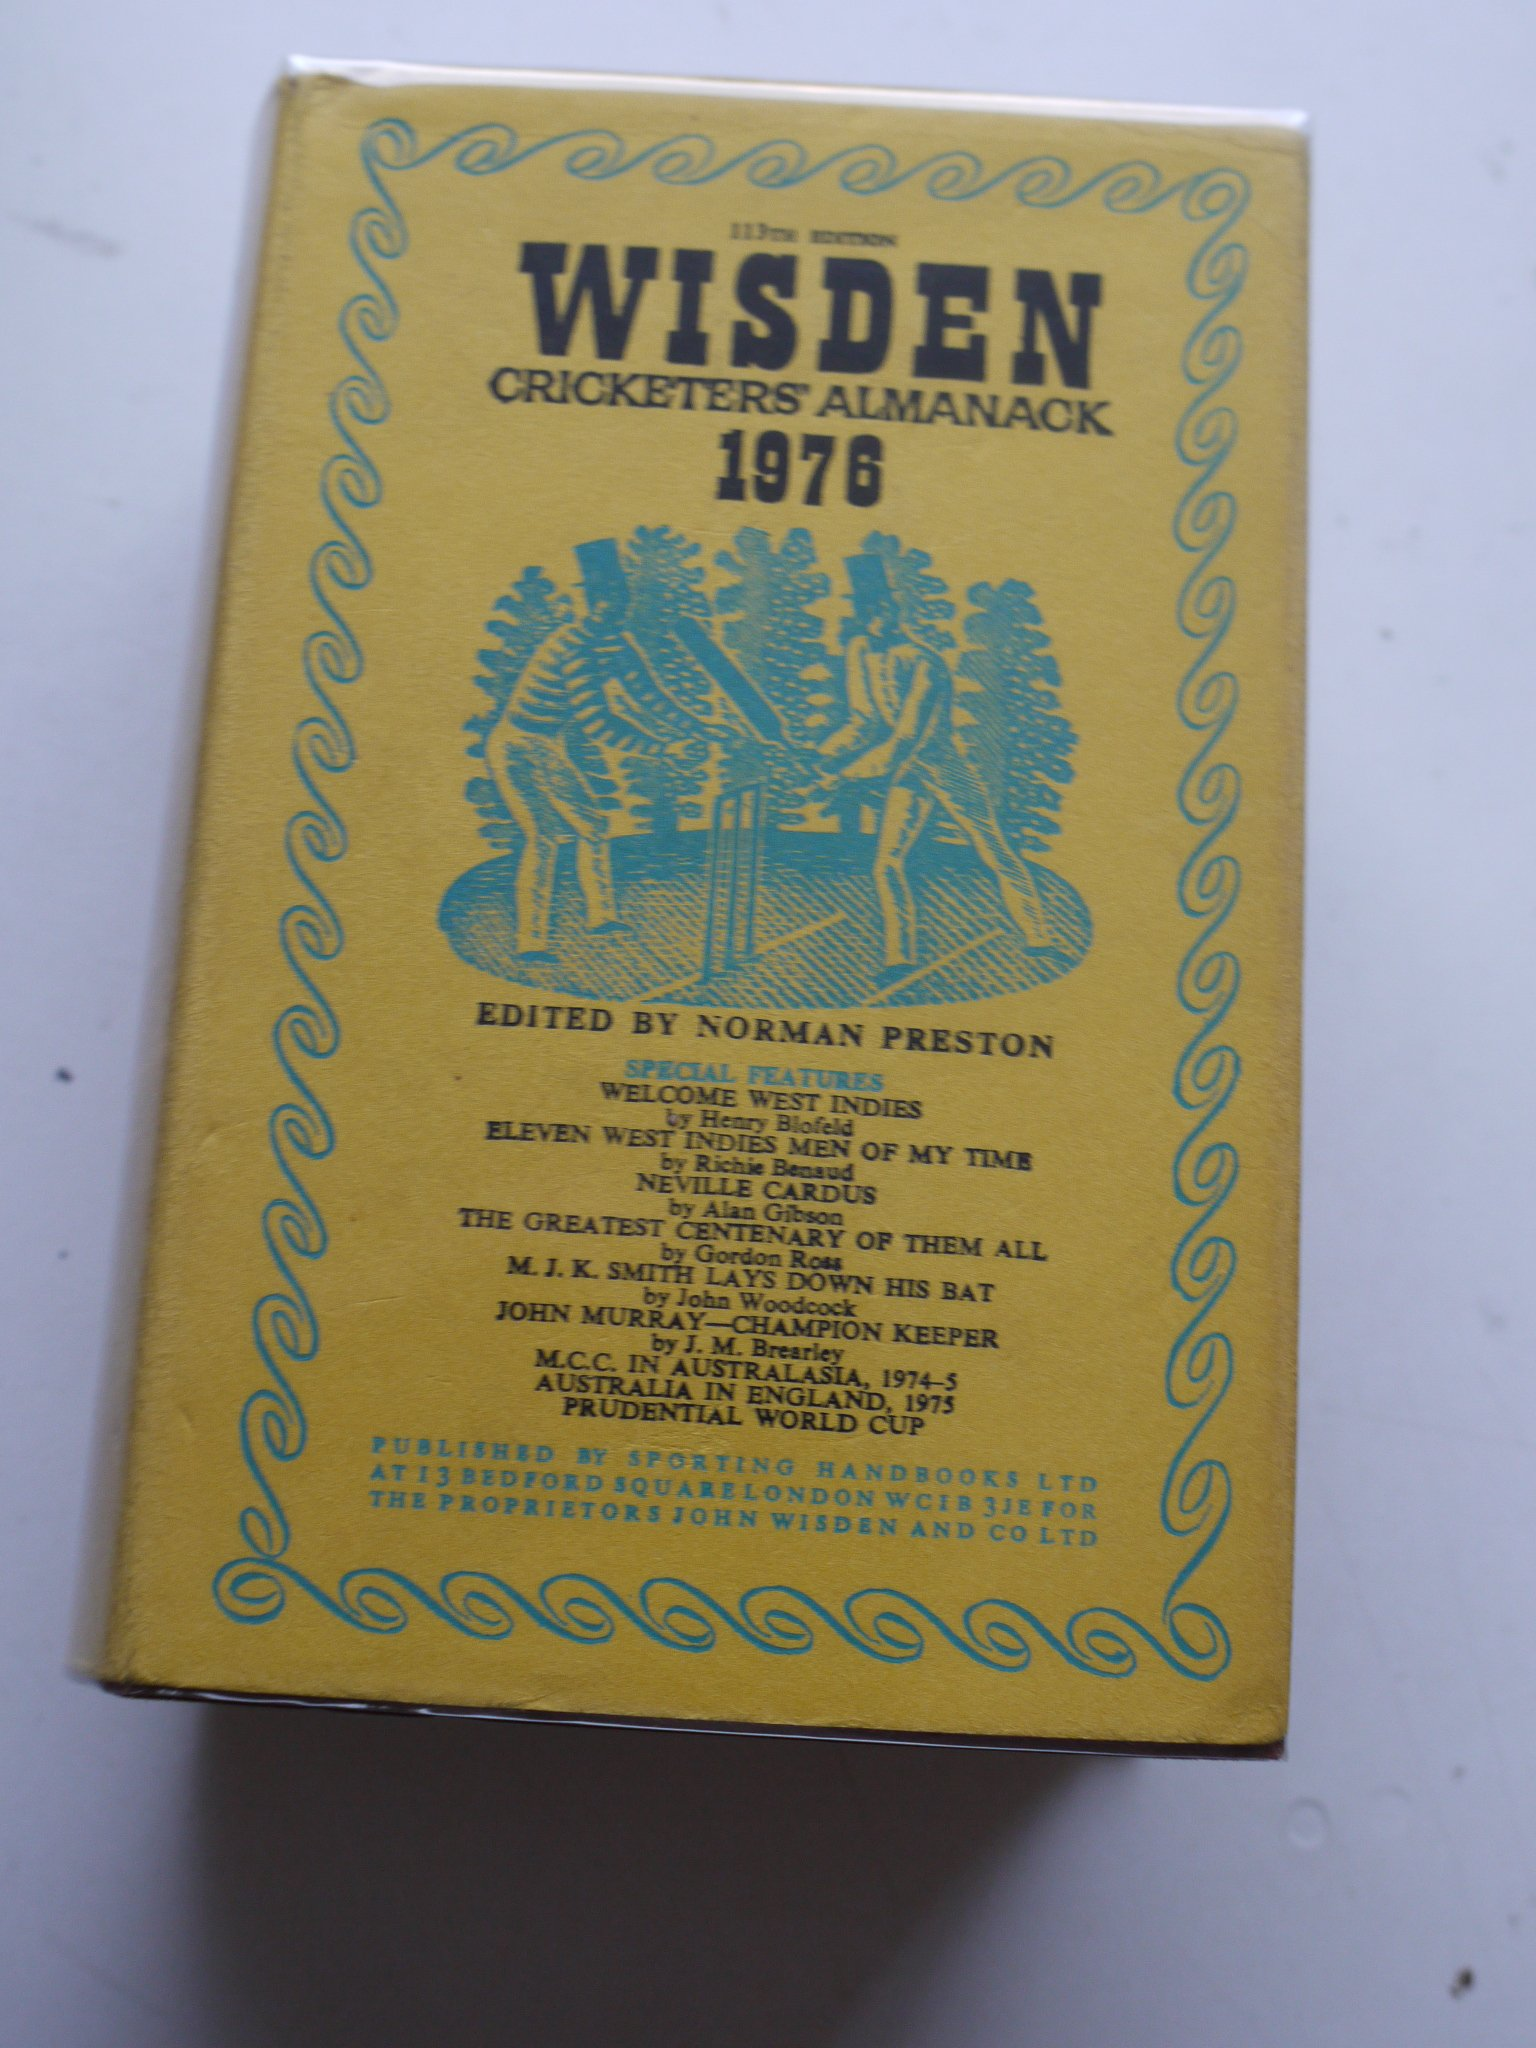
\includegraphics[width=0.45\textwidth, keepaspectratio]{imgs/wisden.jpg}
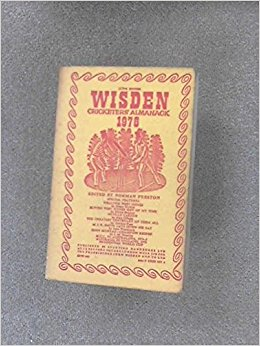
\includegraphics[width=0.45\textwidth, keepaspectratio]{imgs/wisden-paper.jpg}
\end{figure}
\begin{itemize}
\item With propositional logic, the answer is yes.
\begin{itemize}
\item $P$: other customer ordered paperback
\item $H$: other customer ordered hardback
\item $BP$: we can buy the paperback
\item $BH$: we can buy the hardback
\end{itemize}
The other customer ordered one but not both, so it follows that:
\begin{itemize}
\item $P \rightarrow BH$
\item $H \rightarrow BP$
\item $P \leftrightarrow \neg H$
\end{itemize}
This gives the result $BP \vee BH$, so we can buy either the hardback or the paperback.
\item However, if we use constructive logic, it is not enough to know something is true, we have to able to \textit{prove} it and the proof must be ``constructive". For example if we want to prove $P \vee Q$, we must \textit{either} be able to prove $P$ or be able to prove $Q$. Following the Wisden example, it is not enough to know $BP \vee BH$, we have to know \textit{which} one:
\begin{itemize}
\item We can't prove $BP$ because $P$ might be true
\item We can't prove $BH$ because $H$ might be true
\item So we can't give a constructive proof of $BP \vee BH$
\end{itemize}
\end{itemize}
In this example, constructive logic is a better match to reality as the bookseller cannot s
By this logic system, the result is that we \textit{cannot} buy either version of the book.ell either copy because he had to keep them both for the other customer to get whichever he wanted. 
\end{enumerate}
\subsubsection{Entailment}
To talk about logical reasoning, we can use the concept of \textbf{logical entailment} between sentences. The idea is that a sentence \textit{follows logically} from another sentence and can be written as:
\begin{equation}
\alpha\ \vDash \beta
\end{equation}
This means that the sentence $\alpha$ entails the sentence $\beta$. The formal definition of entailment is \textbf{$\alpha \vDash \beta$ if and only if, in every model in which $\alpha$ is true, $\beta$ is also true}. 
\n
Now, if we have some \textbf{Knowledge base} ``KB" of a set of sentences in either propositional or first order logic, and another sentence S in that logic system, it can be said that $KB \vDash S$. So in any interpretation of any model that makes KB true, S must also be true.
\n
The symbol \vdash is the \textit{single turnstile} and represents \textbf{syntactic entailment} whereas the \vDash (double turnstile) represents \textbf{semantic entailment}.
\n
\textbf{Syntactic entailment:} $\alpha \vdash \beta$ says that a sentence $\beta$ is \textit{provable} from the set of assumption $\alpha$. 
\\
\textbf{Semantic entailment:} $\alpha \vDash \beta$ says that a sentence is \textit{true} in all models of $\alpha$.
\n
G\"{o}del's \textbf{Completeness} theorem proved that for the right set of inference rules, if $KB \vDash S$ then $KB \vdash S$. In other words, if something is true in all models then we can prove it. We say that the set of inference rules is \textit{complete}. For the reverse case we also need that if $KB \vdash S$ then $KB \vDash S$. This is called \textbf{soundness} and is usually easier to prove than completeness.
\subsection{Propositional logic}
\textbf{Propositional logic} is a logic system that studies ways of joining and/or modifying entire propositions, statements or sentences to form more complicated propositions, statements or sentences, as well as the logical relationship and properties that are derived from these methods of combining or altering statements. 
\subsubsection{Syntax}
\textbf{Atomic sentences} in propositional logic consist of a single \textbf{propositional symbol}. Each symbol represents a propositions that can either be true or false. Symbols start with an uppercase and may contain subscripts and other letters, for example: $P$, $Q$, $R_{1,2}$, $W_{s}$ and $West$. These symbols are usually arbitrary but can have mnemonic value. \textit{True} is the always true proposition and \textit{False} is the always false proposition. There are also five commonly used \textbf{logical connectives} to connect propositions:
\begin{figure}[H]
\centering
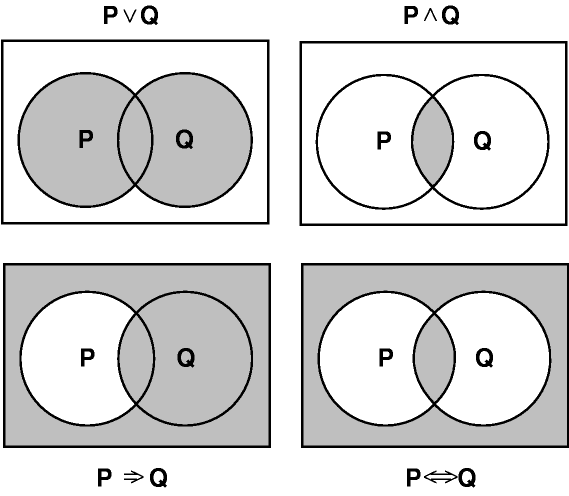
\includegraphics[width=0.7\textwidth, keepaspectratio]{imgs/propositional-symbols.png}
\end{figure}
\begin{itemize}[label={}]
\item $\neg$ (not). This is the \textbf{negation}, for example $\neg P$ is the negation of $P$. A \textbf{literal} is either an atomic sentence (positive literal) or a negative atomic sentence (negative literal). 
\item $\wedge$ (and). This is called a \textbf{conjunction}. For example $P \wedge Q$ is a conjunction of the literals P and Q. It can be thought of as the AND logic gate.
\item $\vee$ (or). This is called a \textbf{disjunction}, we can be thought of as the OR logic gate.
\item $\oplus$ (xor). Just like the XOR logic gate, this is an exclusive OR. 
\item $\rightarrow$ (implies). A sentence such as $P \rightarrow Q$ is called an \textbf{implication}. Implications are also known as \textbf{if-then} statements. $p \rightarrow q$ is logically equivalent to $\neg (p \wedge \neg q)$ and by De Morgan's law equivalent to $\neg p \vee q$. 
\end{itemize}
Two propositional formulae, $A$ and $B$ are called \textbf{equivalent} if $A\leftrightarrow B$ is a \textbf{tautology}. The symbol $\leftrightarrow$ stands for \textbf{if and only if}. A logic formula can also have properties which can be one or more of the following:
\begin{itemize}
\item \textbf{Valid} or \textbf{Tautology} - Every way of assigning the variables true or false makes the formula true
\item \textbf{Invalid} - Not valid, there is at least one assignment which makes the formula untrue
\item \textbf{Satisfiable} - At least one assignment of true/false that makes the formula true. It follows then that all valid formulae are also satisfiable.
\item \textbf{Unsatisfiable} - No assignment of true/false can make the formula true.
\end{itemize}
\subsubsection{Conjunctive normal form}
CNF (Conjunctive normal form) is a restricted form of propositional logic formula. By converting propositional logic to CNF, we can make more specialised and efficient algorithms that work only on CNF.
\n
A formula in CNF is a conjunction ($\wedge$) of disjunctions ($\vee$). In other words, all CNF formula follow something like the following:
\begin{equation}
(\neg A \vee B \vee C) \wedge (D \vee E) \wedge (F \vee G \vee \neg H) ...
\end{equation}
Each formula in parenthesis () is a \textbf{clause} and every variable is a \textbf{literal} which can negated. \textit{Any} propositional formula has an \textit{equivalent} CNF. The order of clauses and literals does not matter, nor do any repeats. A CNF including an empty clause (), that is it contains a clause with no literals:
\begin{equation}
(A \vee B) \wedge () \wedge (B \vee \neg C)
\end{equation}
is unsatisfiable (always false). An empty CNF (\textbf{not} empty clause) is a tautology and always true. An empty CNF means an empty \textit{set of clauses}.
\n
There is a simple procedure to follow to convert from any propositional logic formulae to CNF. The steps are as follows:
\begin{enumerate}
\item Eliminate any $\rightarrow$, $\leftrightarrow$, $\oplus$ into $\wedge$, $\vee$ and $\neg$ with the following rules:
	\begin{itemize}
	\item $A \rightarrow B$ becomes $\neg A \vee B$
	\item $A \leftrightarrow B$ becomes $(A \wedge B) \vee (\neg A \wedge \neg B)$
	\item $A \oplus B$ becomes $(A \wedge \neg B) \vee (\neg A \wedge B)$
	\end{itemize}
\item Move any $\neg$ into the brackets using De Morgan's laws:
	\begin{itemize}
	\item $\neg (A \wedge B)$ becomes $\neg A \vee \neg B$
	\item $\neg (A \vee B)$ becomes $\neg A \wedge \neg B$
	\end{itemize}
\item Distribute $\vee$ over $\wedge$ where possible
	\begin{itemize}
	\item $A \vee (B \wedge C)$ becomes $(A \vee B) \wedge (A \vee C)$
	\end{itemize}
\item Finally, clean up any 1s and 0s with the Zero and Unit laws as well as the 0 and 1 complement laws.
	\begin{itemize}
	\item $A \wedge 0 = 0$
	\item $A \wedge 1 = 1$
	\item $A \vee 0 = A$
	\item $A \vee 1 = 1$
	\item $A \wedge \neg A = 0$
	\item $A \vee \neg A = 1$
	\end{itemize}
\end{enumerate}
With the formula in CNF, it is much harder to read, but it can be used as input into resolution algorithms. 

\subsubsection{Reductio ad absurdum}
\textbf{Reductio ad absurdum} is ``reduction to an absurdity". If we deduce false then the original clause set must be unsatisfiable, so we add the \textit{opposite} of what we want to prove and if we deduce the empty clause then the opposite is unsatisfaible. This means that what we wanted to prove originally must be true. 
\subsection{First-Order logic}
While propositional logic allows us to talk about propositions, \textbf{first order logic} allows us to talk about \textit{objects}. Objects can be almost anything, however, they have no semantics are just regarded as atomics. \textbf{Models} in first order logic represent contexts in which we can analyse truth of sentences and \textbf{interpretations} tell us how to interpret sentences in the context of a model. Therefore \textbf{sentences} are true or false \textit{with respect} to a model and an interpretation.
\subsubsection{Syntax}
The basic syntactic elements of first order logic are the symbols that stand for objects, relations and functions. There are three kinds of symbols:
\begin{enumerate}
\item \textbf{Constant symbols} - which stand for objects
\item \textbf{Predicate symbols} - which stand for relations
\item \textbf{Function symbols} - which stand for functions
\end{enumerate}
A \textbf{function} is simply a mapping between objects, for example \texttt{g(that\_cat) = that\_chair}. A function can have any finite number of arguments including zero arguments. Strictly speaking, functions must be \textbf{total functions}, which means there must be a definite atom for any set of inputs. This can be a bit problematic because sometimes we don't want this. For example if we have a function $LeftLeg()$ that takes as input any object as maps its left leg to it, then each left leg object must also have a valid mapping in this function but that does not make sense. The solution to this is to have an ``invisible" object that is not anything really which the functions always map to in any other case. 
\n
A \textbf{predicate} in first order logic is a statement that may be true or false depending on the values of its variables. So it is like a truth function or a relation. It is like a function and can have multiple arguments. An example predicate would be: 
\begin{equation}
P(X,Y)\text{: true iff the object X is directly above object Y}
\end{equation}
For any set of inputs, the result of the predicate must be either true of false.
\begin{figure}[H]
\centering
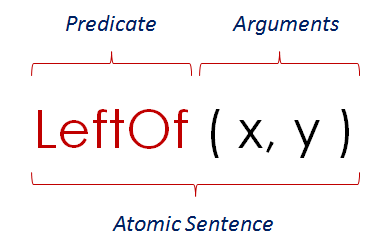
\includegraphics[width=0.6\textwidth, keepaspectratio]{imgs/predicate.png}
\end{figure}
\noindent
Below is the entire basic syntax of first order logic in Backus-Naur form:
\begin{grammar}
<Sentence> $\rightarrow$ <AtomicSentence> | <ComplexSentence>

<AtomicSentence> $\rightarrow$ <Predicate>
\alt <Predicate>(<Term>,...)
\alt <Term> = <Term>

<ComplexSentence> $\rightarrow$ (<Sentence>)
\alt [<Sentence>]
\alt $\neg$ <Sentence>
\alt <Sentence> $\wedge$ <Sentence>
\alt <Sentence> $\vee$ <Sentence>
\alt <Sentence> $\Rightarrow$ <Sentence>
\alt <Sentence> $\Leftrightarrow$ <Sentence>
\alt <Quantifier> <Variable>, ... <Sentence>

<Term> $\rightarrow$ <Function>(<Term>,...)
\alt <Constant>
\alt <Variable>

<Quantifier> $\rightarrow$ $\forall$ | $\exists$

<Constant> $\rightarrow$ A | $X_{1}$ | John | ...

<Variable> $\rightarrow$ $a$ | $x$ | $s$ | ...

<Predicate> $\rightarrow$ \textit{True} | \textit{False} | \textit{Raining} | \textit{P} | ...

<Function> $\rightarrow$ \textit{f()} | \textit{LeftLeg(x)} | ...
\end{grammar}
A \textbf{term} is something that refers to an object. Constant symbols are therefore terms but it is not always convenient to have a distinct symbol to name every object. There are three kinds of terms:
\begin{itemize}
\item \textbf{Constant/Atomic term} - a constant that is on its own
\item \textbf{Variable} - a variable that is on its own
\item \textbf{Compound term} - a function of other terms, i.e, \textit{function(term)}. It can be arbitrarily nested, but it still just denotes one object.
\end{itemize}
\textbf{Equality} where $a = b$ is true iff the object referred to by $a$ is the \textit{same} object as the object referred to by $b$.
\n
There are also two kinds of \textbf{sentences}:
\begin{itemize}
\item \textbf{Atomic sentence} - an atomic sentence (or atom) is formed from a predicate symbol optionally followed by a parenthisised list of terms such as \textit{Brother(Richard, John)}. In other words, a predicate applied to the correct number of terms. Atomic sentences can also have complex terms as arguments, such as \textit{Married(Father(Richard), Mother(John)}. The key is that an atomic sentence is \textbf{true} in a given model if the relation referred to by the predicate symbol holds among the objects referred to by the arguments.
\item \textbf{Complex sentence} - a complex sentence is made from other sentences using connectives. Each sentence is true or false so we can use \textbf{logical connectives} like in propositional logic to connect the sentences. There is also a final form of complex sentence that uses \textbf{quantifiers}.
\end{itemize}
\textbf{Quantifiers} can be used to make new sentences. It lets us express properties of entire collections of objects, instead of just enumerating the objects by name. There are two standard quantifiers in first order logic: \textbf{universal} ($\forall$) and \textbf{existential} ($\exists$).
\n
The \textbf{universal quantifier} ($\forall$) is used for sentences such as ``All kings are persons". That statement can be written in first order logic as:
\begin{equation}
\forall x\ King(x) \Rightarrow Person(x)
\end{equation}
In English, this would mean ``For all $x$, if $x$ is a king, then $x$ is a person." In essence, the sentence $\forall x\ P$ where $P$ is any logical expression, says that $P$ is true for \textit{every} possible value of $x$. The truth table definition of $\Rightarrow$ is perfect for writing general rules with universal quantifiers as we can say ``$x \rightarrow$ the crown" and therefore ``the crown is a king $\Rightarrow$ the crown is a person". This is true because the crown is not a king and therefore not a person. A common mistake is to use $\wedge$ instead of $\Rightarrow$ for universality, giving the statement:
\begin{equation}
\forall x\ King(x) \wedge Person(x)
\end{equation}
This would not be what we want to represent as it gives statements such as:
\begin{equation}
\text{The crown is a king} \wedge \text{The crown is a person}
\end{equation}
\begin{equation}
\text{John's left leg is a king} \wedge \text{John's left leg is a person}
\end{equation}
\n
The \textbf{Existential quantifier} ($\exists$) makes a statement about \textit{some} object in the universe without naming it. For example to say that King John has a crown on his head, it would be:
\begin{equation}
\exists x\ Crown(x) \wedge OnHead(x, John)
\end{equation}
This gives statements that are true iff S(X) is true for \textbf{at least one} possible value of X. In other words, iff S(X) is true when we replace X in it by some object that exists. Just as $\Rightarrow$ is a natural connective for the universal quantifier, $\wedge$ is the natural connective for the existential quantifier. Using $\Rightarrow$ with $\exists$ leads to a very weak statement, for example:
\begin{equation}
\exists x\ Crown(x) \Rightarrow OnHead(x, John)
\end{equation}
leads to the following statements:
\begin{equation}
\text{Richard is a crown} \Rightarrow \text{Richard is on John's head}
\end{equation}
\begin{equation}
\text{John's left leg is a crown} \Rightarrow \text{John's left leg is on John's head}
\end{equation}
Remember, implication is true if both the premise and conclusion are true, \textit{or if the premise is false}. So if the premise ``John's left leg is a crown" is false, then the first assertion is true and the existential is satisfied. So the existential implication is true \textit{whenever any} object fails to satisfy the premise. This is why an implication ($\Rightarrow$) is not suitable for existential quantifiers just like how $\wedge$ is not suitable for universal quantifiers. 
\n
The two quantifiers are actually \textbf{closely connected} with each other through \textbf{negation}. For example, asserting that everyone dislikes pumpkin is the same as asserting there does not exist someone who likes pumpkin and vice versa.
\begin{equation}
\forall x\ \neg Likes(x, Pumpkin) \equiv \neg \exists x\ Likes(x, Pumpkin)
\end{equation}
Further, ``Everyone likes ice cream" means that there is no one who does not like ice cream.
\begin{equation}
\forall x\ Likes(x, IceCream) \equiv \neg \exists x\ \neg Likes(x, IceCream)
\end{equation}
Additionally, $\forall x\ \forall y\ s(x, y)$ \textbf{always} means the same as $\forall y\ \forall x\ s(x, y)$. Similarly, $\exists x\ \exists y\ x(x, y)$ \textbf{always} means the same as $\exists y\ \exists x\ s(x, y)$. However $\exists x\ \forall y\ s(x, y)$ \textbf{often doesn't} means the same as $\forall y\ \exists x\ s(x, y)$. For example, ``Everybody loves somebody" means that for every person, there is someone that person loves.
\begin{equation}
\forall x\ \exists y\ Loves(x, y)
\end{equation}
On the other hand, to say ``There is someone who is loved by everyone" it is
\begin{equation}
\exists x\ \forall y\ Loves(x, y)
\end{equation}
We can see that the order of the quantifications is important as it means different things with different order. Putting parenthesis around the equations helps makes this clearer, i.e.
\begin{equation}
\exists x\ (\forall y\ Loves (x, y))
\end{equation}
\subsubsection{CNF in first order logic}
CNF also turns out to be useful in first order logic, and we can convert sentences from first order logic to CNF in a similar way to how we did it for propositional logic, this allows us to do \textbf{first order resolution}. Unsurprisingly, it is much more complicated. One thing to note is that every sentence in first order logic can be converted into an \textbf{inferentially equivalent} CNF sentence, \textit{not} a fully equivalent CNF sentence. \textbf{Inferentially equivalent} means that the CNF sentence is unsatisfiable iff the original is unsatisfiable. This gives us a basis for proofs by contradiction on the CNF sentences.
\n
The way to convert from first order logic to CNF is similar to the procedure for propositional logic, but we add a few new steps. The main difference is the need to eliminate existential quantifiers. The steps marked in \textcolor{red}{red} are the steps that are in addition to the normal propositional logic procedure.
\begin{enumerate}
\item \textbf{Eliminate implications ($\Rightarrow$)} and any other connectives except for $\wedge \vee \neg$ just like in propositional logic.
\item \textbf{Move negation inwards} just like in propositional logic.
\item \textbf{\textcolor{red}{Standardise quantified variable names apart}}. This is to make sure the same variable name is not used to avoid confusion when quantifiers are dropped. For example
\begin{equation}
(\exists x\ P(x)) \vee (\exists x\ Q(x))\ \text{becomes}\ (\exists x\ P(x)) \vee (\exists y\ Q(y))
\end{equation}
\item \textbf{\textcolor{red}{Skolemise}}. \textbf{Skolemisation} is the process of removing existential quantifiers by elimination. There are two different types of skolemisation:
\begin{itemize}
\item \textbf{Replace with a skolem constant}. This is where we can replace an existential variable X with a \textbf{skolem constant}. For example:
\begin{equation}
\exists X\ norwegian(X) \wedge mathematician(X)\
\end{equation}
becomes
\begin{equation}
norwegian(skolem) \wedge mathematician(skolem)
\end{equation}
This works for any formulae in the form $\exists x\ P(x)$. The \textit{skolem} variable is a \textit{new model} where ``skolem" satisfies the existential sentence.
\item \textbf{Replace with skolem functions}. If the sentence we are trying to convert to CNF does not have an existential in the form $\exists x\ P(x)$, then we must use \textbf{skolem functions} instead of skolem constants. We can think of skolem functions as a function that takes an $X$ as input and returns the object which satisfies the outer function like so:
\begin{equation}
\forall x\ person(x) \Rightarrow \exists y\ mother(x, y)
\end{equation}
becomes
\begin{equation}
\forall x\ person(x) \Rightarrow mother(x, \text{\textbf{skolemf(x)}})
\end{equation}
The general rule is that the arguments of the skolem function (\textbf{skolemf()}) are all the universally quantified variables in whose scope the existential quantifier appears. A Skolemised sentence is satisfiable exactly when the original sentence is satisfiable. 
\end{itemize}
\item \textbf{\textcolor{red}{Drop universal quantifiers}}. At this point, all remaining variables must be universally quantified so we can just drop the universal quantifiers.
\item Finally, \textbf{distribute $\vee$ over $\wedge$} like in propositional logic.
\end{enumerate}
\subsection{Resolution}
\textbf{Resolution} is a \textit{sound} and \textit{complete} proof system that uses first order predicate logic sentences in CNF form. The entire reason to convert first order logic sentences to CNF is to use resolution. The basic idea of resolution is simple, but gets more complicated because of first order logic.

\subsubsection{Resolution in propositional logic}
The basic idea of resolution is we can deduce a new clause from a pair of clauses where remove any \textbf{complementary literals}. Complementary literals are simply literals where one is the identical negation of the other, for example $P$ and $\neg P$. 
\n
Suppose we have the two clauses $(\neg P \vee R)$ and $(P \vee Q)$. We can remove the complementary literals $P, \neg P$ and deduce a new clause $(Q \vee R)$. The result is the \textbf{resolvent clause} or the \textbf{resolvent}. One more aspect of the resolution rule is that the resulting clause should only contain one copy of each literal. For example if we resolve $(A \vee B)$ with $(A \vee \neg B)$, we get $(A \vee A)$ which is just $A$. With resolution, for any sentences $\alpha$ and $\beta$ in propositional logic, we can decide whether $\alpha \vDash \beta$. 
\n
To show that $KB \vDash \alpha$, we show that $(KB \wedge \neg \alpha)$ is unsatisfiable, that is the resolution of $(KB \wedge \neg \alpha)$ is the empty clause. The steps for this algorithm are as follows:
\begin{itemize}
\item Given $KB$ and $\alpha$ in CNF form, create the clause set \textbf{$CS$} where $CS = KB \cup \neg \alpha$
\item Repeat:
	\begin{itemize}
	\item Pick any pair of clauses $C_{1}$ and $C_{2}$ from $CS$
	\item If it is not a tautology, then create the resolvent clause of the pair and add it to $CS$
	\end{itemize}
\item Until:
	\begin{itemize}
	\item Either a resolvent clause is the empty clause
	\item There are no possible resolvents that are not already in CS
	\end{itemize}
\item If we found an empty clause, we have proved $KB \vDash \alpha$
\item If we ran out of resolvents, we have proved $KB \nvDash \alpha$
\end{itemize}
\subsubsection{Resolution in first order logic}
Resolution is first order predicate logic is more complicated than in propositional logic. The key complication is the addition of the \textit{quantified variables}. First order literals are complementary is one \textbf{unifies} with the negation of the other. Below are some examples:
\begin{itemize}
\item $(\neg P(a, b, c)) \wedge P(a, b, c)$ resolves to $()$
\item $(\neg P(a, b, c)) \wedge P(a, c, c)$ cannot be resolves as $b \neq c$
\item $(\neg P(a, b, c)) \wedge P(a, X, c)$ where $X$ is a variable can be resolved to $()$ by setting $X = b$
\item Similarly, $(\neg P(a, skolf(b), c)) \wedge P(a, X, c)$ can also be resolved by setting $X = skolf(b)$
\item $(\neg P(a, b, c)) \wedge P(a, X, X)$ cannot be resolved as $X$ can only be set to either $b$ or $c$, not both.
\item $(\neg P(Y, f(Y), f(f(Y))) \wedge P(a, X, f(X))$ can be resolved by setting $Y = a$ and $X = f(a)$
\end{itemize}
\section{Bayesian probabilistic reasoning}
Sometimes, logical agents have to handle \textit{uncertainty}, either due to partial observation, non-determinism or a combination. For example, consider a simple logical rule:
\begin{equation}
Toothache\ \Rightarrow\ Cavity
\end{equation}
However this rule is wrong, not all people with toothaches have cavities. Some might have a gum disease or another problem. This is a problem as we would need to add an almost unlimited list of possible problems. We could  turn the rule into a causal rule, that is:
\begin{equation}
Cavity\ \Rightarrow\ Toothache
\end{equation}
But this rule isn't right either as not all cavities cause pain. The issue with either rule is we would need to make it exhaustive. Trying to use logic for this is therefore quite difficult for the following reasons:
\begin{itemize}
\item \textbf{Laziness} - It requires too much work to complete the list
\item \textbf{Theoretical ignorance} - Not having enough of a complete theory for the domain
\item \textbf{Practical ignorance} - Even if we know all the rules, we might be uncertain about a particular case
\end{itemize}
The connection in our rule therefore does not follow a logical consequence in either direction. The agent's knowledge can only provide at best a \textbf{degree of belief}. The tool we can use to deal with these degrees and beliefs and uncertainties is \textbf{probability theory}.
\subsection{Probability theory}
We can go through probability theory with a simple example of a dice roll. To roll a six-sided dice, what is the probability it ends up showing a 6?
\begin{equation}
P(d = 6) = \frac{1}{6}
\end{equation}
Probability theory does not require complete knowledge of the probabilities of each possible world. All probabilities in our world range from 0 to 1 and always sum to 1. It doesn't make sense to have a probability greater than 1, that is it is \textit{more} than certain the event will occur. Probabilities can also be added with simple arithmetic, for example, what is the probability that it shows a 1 or a 6?
\begin{equation}
P(d = 1) + P(d = 6) = \frac{1}{6} + \frac{1}{6} = \frac{2}{6}
\end{equation}
\subsubsection{Definitions}
\begin{itemize}
\item An \textbf{event A} is any subset of the sample space $\Omega$, for example A = {1,3,5} is an event of rolling an odd number.
\item Each $\omega$ in $\Omega$ is an \textbf{atomic event}. For example in the set {1,2,3,4,5,6} the possible events for $\omega$ are 1, 2, 3, 4, 5, 6.
\item A \textbf{random variable (r.v.)} is a function from the sample space to some set of values. For example r.v. Odd would be Odd(1)=Odd(3)=Odd(5) = true and others = false.
\item A \textbf{Proposition} is used to refer to the event where the underlying random variable is true, for example $P(Odd) = 0.5$. We can then combine propositions using logical connections like in propositional logic like $P(Odd \vee Even) = 1$ or $(P(Odd \wedge Even) = 0$
\end{itemize}
\subsubsection{Kolmogorov's Axioms for Probability}
\begin{enumerate}
\item All probabilities are between 0 and 1. In other words for any event A, $0 \leq P(A) \leq 1$.
\item Probability of truth = 1, Probability of false = 0.
\item Negation is defined as $P(\neg a) = 1 - P(a)$
\item Sum rules probabilities is as follows:
\begin{equation}
P(a \vee b) = P(a) + P(b) - P(a \wedge b)
\end{equation}
\end{enumerate}
Particular to note is Kolmogorov's fourth axiom. This can be illustrated in a Venn diagram.
\begin{figure}[H]
\centering
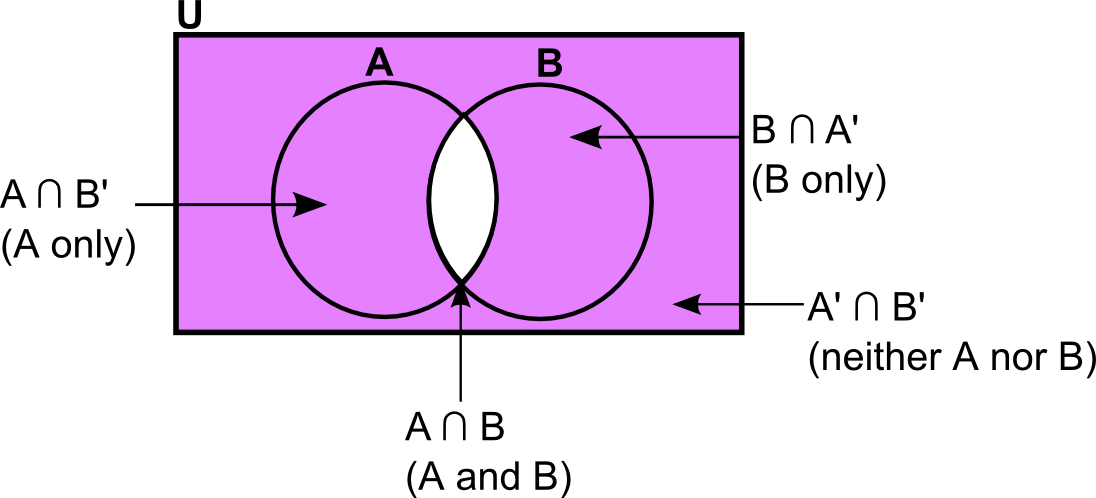
\includegraphics[width=0.8\textwidth, keepaspectratio]{imgs/kolmogorov-fourth.png}
\end{figure}
\noindent
The area which is either in A or B is the area of A + the area of B - the area of A and B to avoid counting it twice. This is a typical inclusion-exclusion result.
\subsubsection{Conditional probability}
We can go through probability theory with a simple example of a dice roll. To roll a six-sided dice, what is the probability it ends up showing a 6?
Probabilities such as $P(d = 1)$ are called \textbf{unconditional} or \textbf{prior} probabilities. This refers to degrees of belief in propositions \textit{in the absence of any other information}. However, usually we have some information, or \textbf{evidence}. For example if we are rolling two dice, the first die may already be showed as a 5 and we are waiting for the next die. In this case, we are not interested in the unconditional probability of rolling doubles, but the \textbf{conditional} or \textbf{posterior} probability of rolling doubles \textit{given} that the first die is a 5. This probability would then be written as:
\begin{equation}
P(doubles | d_{1} = 5)
\end{equation}
This is pronounced probability of doubles \textit{given} the first dice is a 5. They assertion that $P(doubles | d_{1} = 5) = 0.06$ does \textit{not} mean that ``Whenever \textit{doubles} is true, conclude that $d_{1}$ is true with probability 0.06". Instead, it means that ``Whenever  $d_{1} = 5$ is true and \textit{we have no further information}, conclude that \textit{doubles} is true with probability 0.06". This extra condition is important. For example if we had the further information that $doubles$ was not rolled, we would get the equation $P(doubles | d_{1} = 5 \wedge \neg doubles) = 0$.
\n
Conditional probabilities are defined in terms of unconditional probabilities as follows:
\begin{equation}
P(a|b) = \frac{P(a \wedge b)}{P(b)}
\end{equation}
while $P(b) > 0$. A useful alternative formulation of the conditional probability rule is the \textbf{product rule}:
\begin{equation}
P(a \wedge b) = P(a | b)P(b)
\end{equation}
\subsubsection{Probabilistic inference}
The simple method of \textbf{probabilistic inference} is the computation of posterior probabilities for query propositions given observed evidence. We can use a \textbf{full joint distribution} as the knowledge base to answer questions.
\begin{center}
\begin{tabular}{|c|c|c|c|c|}
\hline
& \multicolumn{2}{c|}{\textit{toothache}} & \multicolumn{2}{c|}{$\neg$\textit{toothache}} \\
\hline
& \textit{catch} & $\neg$\textit{catch} & \textit{catch} & $\neg$\textit{catch} \\
\hline
\textit{cavity} & 0.108 & 0.012 & 0.072 & 0.008 \\
\hline
$\neg$\textit{cavity} & 0.16 & 0.64 & 0.144 & 0.576 \\
\hline
\end{tabular}
\end{center}
The domain of the three boolean variables \textit{Toothache}, \textit{Cavity} and \textit{Catch} can be expressed in a table with the probabilities. The sum of the probabilities is 1 as per the axiom and we can directly calculate the probability of any proposition by identifying the possible worlds in which the proposition is true and adding up their probabilities. For example the six possible worlds where $cavity \vee toothache$ is true are:
\begin{equation}
P(cavity \vee toothache) = 0.108 + 0.012 + 0.072 + 0.008 + 0.016 + 0.064
\end{equation}
We can use the rule for conditional probabilities to get an expression in terms of unconditional probabilities and then evaluate the expression from the full joint distribution. For example, we can compute the probability of a cavity, given evidence of a toothache as follows:
\begin{equation}
P(cavity | toothache) = \frac{P(cavity \wedge toothache)}{P(toothache)}
\end{equation}
\subsubsection{Independence}
Suppose we have the probability rule $P(A|B) = P(A)$. This means that the event of $B$ happening does not affect the probability of the event $A$ happening. We can say then that $A$ is \textbf{independent} of $B$. Independence is also equivalent the other way round, if $A$ is independent of $B$, then $B$ is also independent of $A$.
\n
With independence between two events we can get new formulations for the previous conditional rules:
\begin{equation}
P(A|B) = P(A)\ \text{or}\ P(A \wedge B) = P(A)P(B)
\end{equation}
Of course this rule can be continually expanded to more variables provided they are all independent of each other. 
\begin{equation}
P(A \wedge B \wedge C \wedge ... \wedge Z) = P(A)P(B)P(C)...P(Z)
\end{equation}
A key thing to understand about probability is that it is \textit{not} about causation.
\begin{figure}[H]
\centering
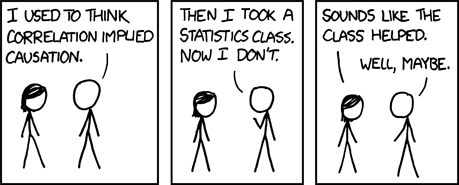
\includegraphics[width=0.8\textwidth, keepaspectratio]{imgs/correlation.png}
\end{figure}
\noindent
An intuitive example is given $P(\neg cavity|toothache) = 0.4$, we don't think that having a toothache has a 0.4 chance of \textit{causing} one not to have a cavity. 
\subsection{Bayes' Rule}
The equation for \textbf{Bayes' rule} is as follows:
\begin{equation}
P(A|B) = \frac{P(B|A)P(A)}{P(B)}
\end{equation}
Those the rule may not seem very useful, it allows us to compute the single term $P(A|B)$ in terms of the three terms: $P(B|A), P(B), P(A)$. We can often perceive as evidence the \textit{effect} of some unknown \textit{cause} and we would like to determine that cause. So then Bayes' rule becomes:
\begin{equation}
P(cause|\text{\textit{effect}}) = \frac{P(\text{\textit{effect}}|cause)P(cause)}{P(\text{\textit{effect}})}
\end{equation}
The conditional probability $P(\text{\textit{effect}}|cause)$ quantifies the relationship in the \textbf{causal} direction, whereas $P(cause|\text{\textit{effect}})$ describes the \textbf{diagnostic} direction. For example in medical diagnosis, we often have conditional probabilities on causal relationships, that is $P(disease|symptoms)$.
\n
It is often easier in practice to compute \textit{causal conditional probabilities}, for example what is the probability that I have these symptoms given I have this disease. Then, what we want is to compute the \textit{diagnostic conditional probabilities}, for example what is the probability that I have this disease given I am showing these symptoms. Most notably, \textit{diagnostic knowledge is more fragile than casual knowledge}. If there is a sudden epidemic of a disease, the probability of the disease (the prior probability) will increase and therefore the diagnostic probability ($P(disease|symptoms)$) will increase. However the casual information $P(symptoms|disease)$ remains unaffected by the epidemic, because it simply reflects the way the disease works.
\subsubsection{Combining evidence and conditional independence}
Now that we have seen Bayes' rule with one piece of evidence, we can explore what happens when we are giving two or more pieces of evidence. In the toothache example, what can we conclude given more evidence?
\begin{equation}
P(cavity|toothache \wedge catch) = \frac{P(toothache \wedge catch | cavity)P(cavity)}{P(toothache \wedge catch)}
\end{equation}
For this to work, we need to know the conditional probabilities of the conjunction $toothache \wedge catch$ for each value of $cavity$. This might be feasible for two values, but it does not scale up to more. Rather than have large full join distributions and read off the table, we can use the concept of independence again.
\n
It would be nice if \textit{toothache} and \textit{catch} were independent, but they are not. However, these variables \textit{are} independent \textit{given the presence or absence of a cavity}. In other words, each is directly caused by the cavity, but neither has a direct effect on the other. We can express this in the following equation:
\begin{equation}
P(toothache \wedge catch | cavity) = P(toothache|cavity)P(catch|cavity)
\end{equation}
This is known as \textbf{conditional independence} of \textit{toothache} and \textit{catch} given \textit{cavity}. Now we can substitute is back into our Bayes' equation and get
\begin{equation}
P(cavity|toothache \wedge catch) 
= \frac{P(toothache|cavity)P(catch|cavity)P(cavity)}{P(toothache \wedge catch}
\end{equation}
\\
The general definition of \textbf{conditional independence} of two variables A and B, given a third variable C is as follows:
\begin{equation}
P(A \wedge B | C) = P(A|C)P(B|C)
\end{equation}
Conditional independence allows probabilistic systems to scale up to more variables. Moreover, they are more commonly available than absolute independence assertions. Conceptually, \textit{cavity} \textbf{separates} \textit{toothache} and \textit{cavity} because it is a direct cause of both of them. 

\subsection{Bayesian Networks}
We saw previously that a full joint probability distribution can answer any question about the domain, but it does not scale well with a larger number of variables. Furthermore it is tedious to specify possible worlds one by one. \textbf{Independence} and \textbf{conditional independence} can help reduce the number of probabilities that need to be specified to define the full joint distribution.
\n
With that in mind, we can introduce a new data structure to represent dependencies among variables: a \textbf{Bayesian network}. A Bayesian network can represent any full join probability distribution as a directed graph in which each node is annotated with quantitative probability information. The full specification is as follows:
\begin{itemize}
\item Each node corresponds to a random variable, which can be discrete or continuous.
\item A set of arrows (directed links) connects pairs of node. An arrow from node X to node Y says that X is the \textit{parent} of Y. The graph has no directed cycles and so is called a \textbf{directed acyclic graph} or DAG.
\item Each node $X_{i}$ has a conditional probability distribution $P(X_{i}|Parents(X_{i}))$ that quantifies the effect of the parents on the node
\end{itemize}
The set of nodes and links in the network specifies the conditional independence relationships that hold in the domain. An arrow between X and Y means that X has a \textit{direct influence} on Y. If nodes do not have an arrow between them, that is to say they independent or conditionally independent. 
\begin{figure}[H]
\centering
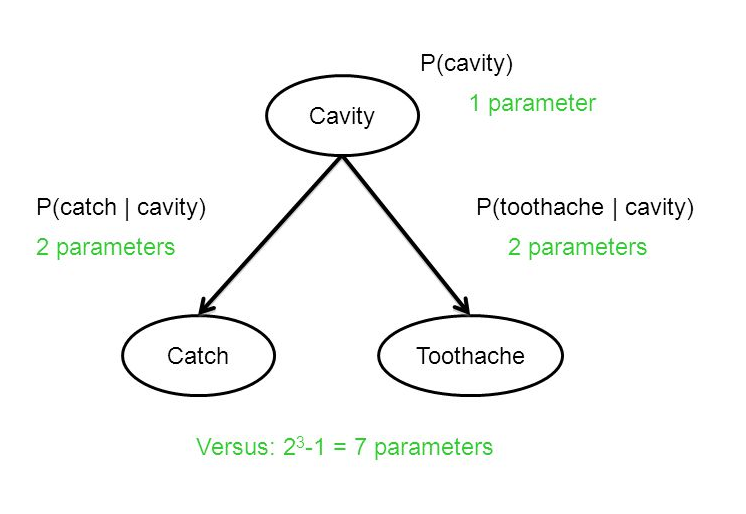
\includegraphics[width=0.9\textwidth, keepaspectratio]{imgs/toothache-bayes-network.png}
\end{figure}
\noindent
In our toothache example, the conditional independence of \textit{Toothache} and \textit{Catch} given \textit{Cavity} is expressed from the topology of the network. The absence of a link between \textit{Toothache} and \textit{Catch} indicates the conditional independence. The network therefore represents the fact that \textit{Cavity} is a direct cause of \textit{Toothache} and \textit{Catch}, but there is no direct causal relationship between \textit{Toothache} and \textit{Catch}.
\n
Let's consider another example of earthquakes and burglaries:
\begin{displayquote}
\textit{We have a new burglar alarm installed at home. It is fairly reliable at detecting a burglary, but also respond on occasion to minor earthquakes. We also have two neighbours, John and Mary, who have promised to call us if they hear the alarm. John nearly always calls, but sometimes confuses the telephone ringing with the alarm and calls then too. Mary, on the other hand, often misses the alarm altogether. Given the evidence of who has or has not called, we would like to estimate the probability of a burglary.}
\end{displayquote}
\noindent
Our network structure should show how burglary and earthquakes direct affect the probability of the alarm going off, and whether John or Mary calls depends only on the alarm. Further, their calling is not affect by the burglaries or earthquakes directly. 
\begin{figure}[H]
\centering
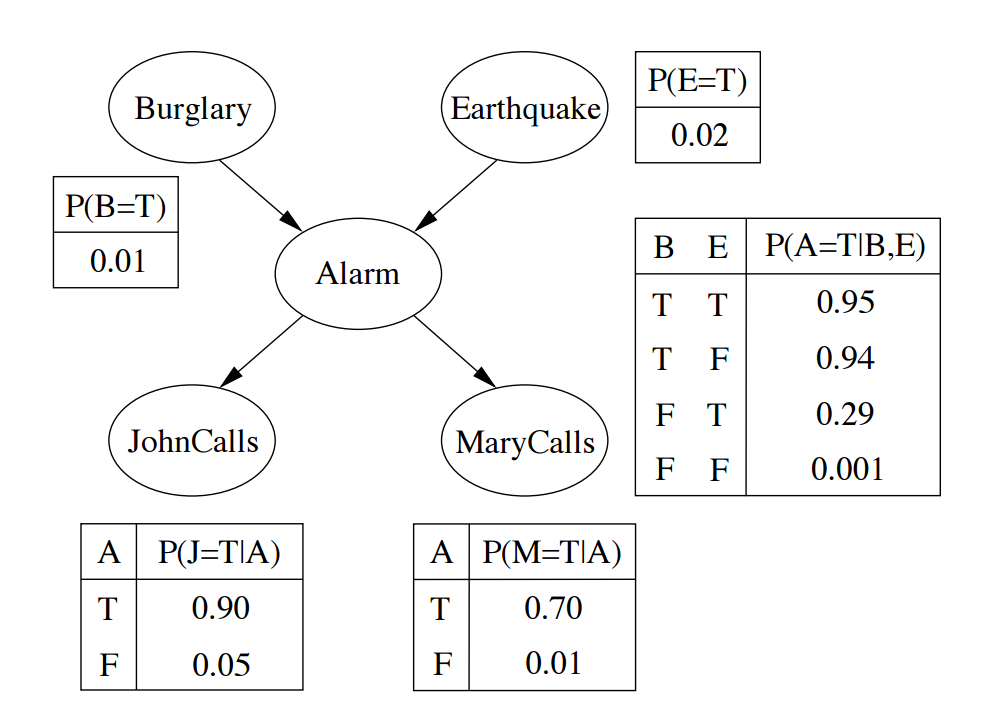
\includegraphics[width=0.9\textwidth, keepaspectratio]{imgs/burglar-bayes-network.png}
\end{figure}
\noindent
The tables in the network are \textbf{conditional probability tables}. Each row in the table contains the conditional probability of each node value for a \textbf{conditioning case}. A conditioning case is just a possible combination of values for the parent nodes. The cases should be exhaustive, however once the probability of a true value \textit{p} is known, the false value is simply $1 - p$ and so we can omit the second value. 

\subsubsection{Constructing Bayesian networks}
Now we must learn how to \textit{construct} Bayesian networks so that the resulting joint distribution is a good representation of a given domain. A Bayesian network is a correct representation of the domain only if each node is conditionally independent of its other predecessors in the node ordering, given its parents. This gives the following methodology for constructing new networks:
\begin{enumerate}
\item \textit{Nodes}: First determine the set of variables that are required to model the domain, the order them ${X_{1}, ..., X_{n}}$. Any order orders, however more compact networks will be created if the ordering is such that causes precede effects.
\item \textit{Links}: For $i = 1$ to $n$ do:
	\begin{itemize}
	\item Choose from $X_{1}, ... X_{i-1}$, a minimal set of parents for $X_{i}$ such that the equation $P(X_{i}|X_{i-1},...,X_{1}) = P(X_{i}|Parents(X_{i}))$ is satisfied
	\item For each parent insert a link from the parent to $X_{i}$
	\item \textit{CPTs}: Write down the conditional probability table $P(X_{i}|Parents(X_{i}))$
	\end{itemize}
\end{enumerate}

\end{document} 